%% History:
% Pavel Tvrdik (26.12.2004)
%  + initial version for PhD Report
%
% Daniel Sykora (27.01.2005)
%
% Michal Valenta (3.12.2008)
% rada zmen ve formatovani (diky M. Duškovi, J. Holubovi a J. Žďárkovi)
% sjednoceni zdrojoveho kodu pro anglickou, ceskou, bakalarskou a diplomovou praci

% One-page layout: (proof-)reading on display
%%%% \documentclass[11pt,oneside,a4paper]{book}
% Two-page layout: final printing
% openany - kapitoly bez vynechání stránky
\documentclass[11pt,twoside,a4paper]{book}   
%=-=-=-=-=-=-=-=-=-=-=-=--=%
% The user of this template may find useful to have an alternative to these 
% officially suggested packages:
\usepackage[czech, english]{babel}
\usepackage[T1]{fontenc} % pouzije EC fonty 
% pripadne pisete-li cesky, pak lze zkusit take:
% \usepackage[OT1]{fontenc} 
\usepackage[utf8]{inputenc}
\usepackage{lmodern}
%=-=-=-=-=-=-=-=-=-=-=-=--=%
% In case of problems with PDF fonts, one may try to uncomment this line:
%\usepackage{lmodern}
%=-=-=-=-=-=-=-=-=-=-=-=--=%
%=-=-=-=-=-=-=-=-=-=-=-=--=%
% Depending on your particular TeX distribution and version of conversion tools 
% (dvips/dvipdf/ps2pdf), some (advanced | desperate) users may prefer to use 
% different settings.
% Please uncomment the following style and use your CSLaTeX (cslatex/pdfcslatex) 
% to process your work. Note however, this file is in UTF-8 and a conversion to 
% your native encoding may be required. Some settings below depend on babel 
% macros and should also be modified. See \selectlanguage \iflanguage.
%\usepackage{czech}  %%%%%\usepackage[T1]{czech} %%%%[IL2] [T1] [OT1]
%=-=-=-=-=-=-=-=-=-=-=-=--=%

%%%%%%%%%%%%%%%%%%%%%%%%%%%%%%%%%%%%%%%
% Styles required in your work follow %
%%%%%%%%%%%%%%%%%%%%%%%%%%%%%%%%%%%%%%%
\usepackage{graphicx}
%\usepackage{indentfirst} %1. odstavec jako v cestine.

\usepackage{subfigure}

\usepackage{array}

\usepackage{multirow}

\usepackage{textcomp}
\usepackage[usenames]{color}
\definecolor{lightgray}{gray}{0.95}
\definecolor{Black}{gray}{0.0}
\usepackage{listings}

\renewcommand\lstlistingname{Zdrojový kód}
\renewcommand\lstlistlistingname{Zdrojové kódy}

\lstset{
numbers=left,                   % where to put the line-numbers
numberstyle=\footnotesize,      % the size of the fonts that are used for the line-numbers
backgroundcolor=\color{lightgray},
captionpos=b,
tabsize=2,
rulecolor=,
basicstyle=\footnotesize, %\scriptsize,
upquote=true,
aboveskip={1.5\baselineskip},
columns=fixed,
showstringspaces=false,
extendedchars=true,
breaklines=true,
prebreak = \raisebox{0ex}[0ex][0ex]{\ensuremath{\hookleftarrow}},
frame=bt,
showtabs=false,
showspaces=false,
showstringspaces=false,
identifierstyle=\ttfamily,
keywordstyle=\color[rgb]{1.0,0,0},
keywordstyle=[1]\color[rgb]{0,0,0.75},
keywordstyle=[2]\color[rgb]{0.5,0.0,0.0},
keywordstyle=[3]\color[rgb]{0.127,0.427,0.514},
keywordstyle=[4]\color[rgb]{0.4,0.4,0.4},
commentstyle=\color[rgb]{0.133,0.545,0.133},
stringstyle=\color[rgb]{0.639,0.082,0.082},
}

\lstdefinelanguage{CSharp}
{
sensitive=true,
morekeywords=[1]{
abstract, as, base, break, case,
catch, checked, class, const, continue,
default, delegate, do, else, enum,
event, explicit, extern, false,
finally, fixed, for, foreach, goto, if,
implicit, in, interface, internal, is,
lock, namespace, new, null, operator,
out, override, params, private,
protected, public, readonly, ref,
return, sealed, sizeof, stackalloc,
static, struct, switch, this, throw,
true, try, typeof, unchecked, unsafe,
using, virtual, volatile, while, bool,
byte, char, decimal, double, float,
int, lock, object, sbyte, short, string,
uint, ulong, ushort, void, set, get, where, var},
morecomment=[l]{//},
morecomment=[s]{/*}{*/},
morecomment=[l][keywordstyle4]{\#},
morestring=[b]",
morestring=[b]',
}




\usepackage{k336_thesis_macros} % specialni makra pro formatovani DP a BP
 % muzete si vytvorit i sva vlastni v souboru k336_thesis_macros.sty
 % najdete  radu jednoduchych definic, ktere zde ani nejsou pouzity
 % napriklad: 
 % \newcommand{\bfig}{\begin{figure}\begin{center}}
 % \newcommand{\efig}{\end{center}\end{figure}}
 % umoznuje pouzit prikaz \bfig namisto \begin{figure}\begin{center} atd.


%%%%%%%%%%%%%%%%%%%%%%%%%%%%%%%%%%%%%
% Zvolte jednu z moznosti 
% Choose one of the following options
%%%%%%%%%%%%%%%%%%%%%%%%%%%%%%%%%%%%%
\newcommand\TypeOfWork{Diplomová práce} \typeout{Diplomova prace}
% \newcommand\TypeOfWork{Master's Thesis}   \typeout{Master's Thesis} 
% \newcommand\TypeOfWork{Bakalářská práce}  \typeout{Bakalarska prace}
% \newcommand\TypeOfWork{Bachelor's Project}  \typeout{Bachelor's Project}


%%%%%%%%%%%%%%%%%%%%%%%%%%%%%%%%%%%%%
% Zvolte jednu z moznosti 
% Choose one of the following options
%%%%%%%%%%%%%%%%%%%%%%%%%%%%%%%%%%%%%
% nabidky jsou z: http://www.fel.cvut.cz/cz/education/bk/prehled.html

%\newcommand\StudProgram{Elektrotechnika a informatika, dobíhající, Bakalářský}
%\newcommand\StudProgram{Elektrotechnika a informatika, dobíhající, Magisterský}
% \newcommand\StudProgram{Elektrotechnika a informatika, strukturovaný, Bakalářský}
 \newcommand\StudProgram{Elektrotechnika a informatika, strukturovaný, Navazující magisterský}
% \newcommand\StudProgram{Softwarové technologie a management, Bakalářský}
% English study:
% \newcommand\StudProgram{Electrical Engineering and Information Technology}  % bachelor programe
% \newcommand\StudProgram{Electrical Engineering and Information Technology}  %master program


%%%%%%%%%%%%%%%%%%%%%%%%%%%%%%%%%%%%%
% Zvolte jednu z moznosti 
% Choose one of the following options
%%%%%%%%%%%%%%%%%%%%%%%%%%%%%%%%%%%%%
% nabidky jsou z: http://www.fel.cvut.cz/cz/education/bk/prehled.html

%\newcommand\StudBranch{Výpočetní technika}   % pro program EaI bak. (dobihajici i strukt.)
\newcommand\StudBranch{Výpočetní technika}   % pro prgoram EaI mag. (dobihajici i strukt.)
%\newcommand\StudBranch{Softwarové inženýrství}            %pro STM
%\newcommand\StudBranch{Web a multimedia}                  % pro STM
%\newcommand\StudBranch{Computer Engineering}              % bachelor programe
%\newcommand\StudBranch{Computer Science and Engineering}  % master programe


%%%%%%%%%%%%%%%%%%%%%%%%%%%%%%%%%%%%%%%%%%%%
% Vyplnte nazev prace, autora a vedouciho
% Set up Work Title, Author and Supervisor
%%%%%%%%%%%%%%%%%%%%%%%%%%%%%%%%%%%%%%%%%%%%

\newcommand\WorkTitle{Modulární E-shop}
\newcommand\FirstandFamilyName{Bc. Petr Diviš}
\newcommand\Supervisor{Ing. Božena Mannová, Ph.D.}


% Pouzijete-li pdflatex, tak je prijemne, kdyz bude mit vase prace
% funkcni odkazy i v pdf formatu
\usepackage[
pdftitle={\WorkTitle},
pdfauthor={\FirstandFamilyName},
bookmarks=true,
colorlinks=true,
breaklinks=true,
urlcolor=red,
citecolor=blue,
linkcolor=blue,
unicode=true,
]
{hyperref}



% Extension posted by Petr Dlouhy in order for better sources reference (\cite{} command) especially in Czech.
% April 2010
% See comment over \thebibliography command for details.

\usepackage[square, numbers]{natbib}             % sazba pouzite literatury
%\usepackage{url}
%\DeclareUrlCommand\url{\def\UrlLeft{<}\def\UrlRight{>}\urlstyle{tt}}  %rm/sf/tt
%\renewcommand{\emph}[1]{\textsl{#1}}    % melo by byt kurziva nebo sklonene,
\let\oldUrl\url
\renewcommand\url[1]{<\texttt{\oldUrl{#1}}>}

%start kapitol na levé straně
%\makeatletter
%\renewcommand*\cleardoublepage{
%  \clearpage\if@twoside
%     \ifodd\c@page \hbox{}\newpage\if@twocolumn\hbox{}%
%     \newpage\fi\fi\fi
%  }
%\makeatother


\begin{document}

%%%%%%%%%%%%%%%%%%%%%%%%%%%%%%%%%%%%%
% Zvolte jednu z moznosti 
% Choose one of the following options
%%%%%%%%%%%%%%%%%%%%%%%%%%%%%%%%%%%%%
\selectlanguage{czech}
%\selectlanguage{english} 

% prikaz \typeout vypise vyse uvedena nastaveni v prikazovem okne
% pro pohodlne ladeni prace


\iflanguage{czech}{
	 \typeout{************************************************}
	 \typeout{Zvoleny jazyk: cestina}
	 \typeout{Typ prace: \TypeOfWork}
	 \typeout{Studijni program: \StudProgram}
	 \typeout{Obor: \StudBranch}
	 \typeout{Jmeno: \FirstandFamilyName}
	 \typeout{Nazev prace: \WorkTitle}
	 \typeout{Vedouci prace: \Supervisor}
	 \typeout{***************************************************}
	 \newcommand\Department{Katedra počítačů}
	 \newcommand\Faculty{Fakulta elektrotechnická}
	 \newcommand\University{České vysoké učení technické v Praze}
	 \newcommand\labelSupervisor{Vedoucí práce}
	 \newcommand\labelStudProgram{Studijní program}
	 \newcommand\labelStudBranch{Obor}
}{
	 \typeout{************************************************}
	 \typeout{Language: english}
	 \typeout{Type of Work: \TypeOfWork}
	 \typeout{Study Program: \StudProgram}
	 \typeout{Study Branch: \StudBranch}
	 \typeout{Author: \FirstandFamilyName}
	 \typeout{Title: \WorkTitle}
	 \typeout{Supervisor: \Supervisor}
	 \typeout{***************************************************}
	 \newcommand\Department{Department of Computer Science and Engineering}
	 \newcommand\Faculty{Faculty of Electrical Engineering}
	 \newcommand\University{Czech Technical University in Prague}
	 \newcommand\labelSupervisor{Supervisor}
	 \newcommand\labelStudProgram{Study Programme} 
	 \newcommand\labelStudBranch{Field of Study}
}




%%%%%%%%%%%%%%%%%%%%%%%%%%    Poznamky ke kompletaci prace
% Nasledujici pasaz uzavrenou v {} ve sve praci samozrejme 
% zakomentujte nebo odstrante. 
% Ve vysledne svazane praci bude nahrazena skutecnym 
% oficialnim zadanim vasi prace.
{
\pagenumbering{roman} \oldcleardoublepage \thispagestyle{empty}
\begin{figure}
\begin{center}

\includegraphics[width=15cm]{figures/zadani.png}
\end{center}
\end{figure}
\newpage
}

%%%%%%%%%%%%%%%%%%%%%%%%%%    Titulni stranka / Title page 

\coverpagestarts

%%%%%%%%%%%%%%%%%%%%%%%%%%%    Podekovani / Acknowledgements 

\acknowledgements
\noindent
V první řadě bych chtěl poděkovat své vedoucí Ing. Boženě Mannové, Ph.D. za vstřícný přístup, poskytnutí konzultací a její připomínky. Nesmím také zapomenout na Ing. Tomáše Černého, který vedl přínosná cvičení předmětu Architektury softwarových systémů a doporučil nám výbornou literaturu. Dále bych chtěl poděkovat své rodině za podporu a pochopení při studiu i při psaní této práce. V poslední řadě bych chtěl poděkovat všem, kteří pomáhali s opravou pravopisných chyb v této práci.


%%%%%%%%%%%%%%%%%%%%%%%%%%%   Prohlaseni / Declaration 

\declaration{V~Rakovníku dne 1.\,1.\,2012}
%\declaration{In Kořenovice nad Bečvárkou on May 15, 2008}


%%%%%%%%%%%%%%%%%%%%%%%%%%%%    Abstract 
 
\abstractpage
This thesis deals with a working concept of internet e-commerce application, which addapts modular software architecture.  First the research on existing open-source and commercial solutions is done, then the research on programming languages and their development platforms with matching frameworks is performed. After choosing a suitable programming language with a framework the analysis and design of the implementation is described in depth. Then there are described the way of the implementation and necessary compromises when programming into the chosen language platform. After that the comparison with the existing solutions is done. In the conclusion results of the thesis are evaluated, compared with the defined goals and possible extensions of the modular e-commerce are proposed.


% Prace v cestine musi krome abstraktu v anglictine obsahovat i
% abstrakt v cestine.
\vglue60mm

\noindent{\Huge \textbf{Abstrakt}}
\vskip 2.75\baselineskip

\noindent
Tato práce se zabývá internetovým obchodem, který si klade za cíl mít modulární softwarovou architekturu. Nejprve je provedena rešerše mezi již existujícími komerčními i open-source internetovými obchody. Dále rešerše zpracovává výběr ze současných programovacích jazyků s vhodnými frameworky. Po zvolení vhodného programovacího jazyka s frameworkem je provedena analýza a návrh implementace. Poté je popsán způsob implementace a nutné kompromisy při programování do zvoleného jazyka. V dalším bodě práce je implementované řešení otestováno a porovnáno s již existujícími řešeními. V závěru jsou zhodnoceny výsledky práce, porovnány s vytyčenými cíli a je naznačeno další možné pokračování vývoje modulárního e-shopu.


%%%%%%%%%%%%%%%%%%%%%%%%%%%%%%%%  Obsah / Table of Contents 

\tableofcontents


%%%%%%%%%%%%%%%%%%%%%%%%%%%%%%%  Seznam obrazku / List of Figures 

\listoffigures


%%%%%%%%%%%%%%%%%%%%%%%%%%%%%%%  Seznam tabulek / List of Tables

\listoftables


%**************************************************************

\mainbodystarts
% horizontalní mezera mezi dvema odstavci
%\parskip=5pt
%11.12.2008 parskip + tolerance
\normalfont
\parskip=0.2\baselineskip plus 0.2\baselineskip minus 0.1\baselineskip

% Odsazeni prvniho radku odstavce resi class book (neaplikuje se na prvni 
% odstavce kapitol, sekci, podsekci atd.) Viz usepackage{indentfirst}.
% Chcete-li selektivne zamezit odsazeni 1. radku nektereho odstavce,
% pouzijte prikaz \noindent.

%**************************************************************

% Pro snadnejsi praci s vetsimi texty je rozumne tyto rozdelit
% do samostatnych souboru nejlepe dle kapitol a tyto potom vkladat
% pomoci prikazu \include{jmeno_souboru.tex} nebo \include{jmeno_souboru}.
% Napr.:
% \include{1_uvod}
% \include{2_teorie}
% atd...

%start kapitol na levé straně

%*****************************************************************************
\chapter{Úvod}
Internetových obchodů existuje nepřeberné množství. Nakupování na internetu se stalo fenoménem posledních 10ti let a vypadá to, že se bude jen nadále rozšiřovat. Jen v České republice se tržby internetových obchodů za poslední období Vánoc roku 2010 prodalo zboží za přibližně 13 miliard korun a průměrný nárůst obratu oproti období Vánoc z roku 2009 byl neuvěřitelných 40\% \cite{vanocenainternetu}. Od počátku internetového nakupování se toto odvětví neustále rozšiřuje a vyvíjí. Roste s ním nejen kvalita služeb nabízených obchodníky, ale i uživatelská přívětivost internetových obchodů a jejich systémů. To vše díky rychle se vyvíjejícím technologiím a silně konkurenčnímu prostředí internetového podnikání.

Pro tým nebo jednotlivce vyvíjející internetový obchod, ať už jako komerční či open-source produkt, je proto zásadní výběr programového vybavení a platformy, na které bude tento produkt zakládat a rozvíjet. Je třeba počítat s požadavky obchodníků a rychlým vývojem trhu s těmito softwarovými produkty. Nově vznikající webové standardy, inovované vlastnosti programovacích a grafických prostředí rychle prostupují mezi vývojáře a jen ti, kteří dokáží pružně reagovat a tyto novinky nabídnout ve svých produktech, udrží aktuálnost a konkurenceschopnost v moři jiných internetových obchodů.

\section*{Proč modulární?}

Návrh a implementace individuálního řešení internetového obchodu obchodníkům se specifickými požadavky je sice v několika parametrech odlišná, ale hodně parametrů a funkčností má podobných. Práce programátora se tak velice často opakuje i přesto, že pro společné vlastnosti a funkčnost používá kód již hotový, funkční a otestovaný. Roste tak nejen časová náročnost vývoje takového řešení na míru, ale i náklady na vývoj, nemluvě o demotivaci programátora, který musí nevyhnutelné opakující se rutiny provádět znova a znova.

Proto přišla myšlenka dynamicky rozšiřitelného internetového obchodu, který bude schopný rychlejšímu přizpůsobení požadavkům obchodníků a bude možné rozšířit jeho jádro o další funkce a technologie bez většího zásahu v kódu samotného jádra.

Již v úvodu je třeba říct, že tento program není vytvářen za účelem nasazení v komerčním prostředí. Klade si za cíl ověřit, že je tvorba takového modulárního internetového obchodu možná a soustředí se na samotné možnosti rozšiřitelnosti jako takové na vhodně zvolené vývojové platformě.

%TODO: do závěru?
Vývoj finálního produktu pro obchodníky vyžaduje mnohem delší časový interval, více lidských zdrojů, více zkušeností s vývojem internetových aplikací a nadmíru kvalitní znalost vývojového prostředí, do kterého je nutné celý projekt dobře navrhnout a dlouhodobě otestovat. Podle nabytých zkušeností je nejlepší vývoj určený pro ostré produkční prostředí. Vzhledem k tomu, že během této práce probíhalo seznamování se se zvoleným vývojovým prostředím, objevuje se v práci všeobecně známý vývojový fenomén \uv{nalezení lepšího způsobu, když je hotovo}.


\section{Popis struktury práce}
%TODO: zkontrolovat kapitoly
Tato práce představuje popis problému a vymezuje cíle a požadavky v kapitole \ref{sec:popisproblemu}. Kapitola \ref{sec:reserse} provádí rešerši na aktuální nabídku dostupných typových internetových obchodů jak komerčních, tak open-source. Dále provádí rešerši všech vhodných implementačních prostředí. Analýza v kapitole \ref{sec:analyza} se soustředí na systematický rozbor modulárního e-shopu do podstatných detailů, potřebných k nutnému porozumění fungování aplikace e-shopu včetně různých alternativ. V kapitole \ref{sec:analyza} je popsána také volba implementačního prostředí vybraného z prostředí zmíněných v předchozí kapitole \ref{sec:reserse}. V kapitole \ref{sec:realizace} je následně popsána implementace se zaměřením na nestandardní řešení. Implementace využívá vlastností zvolené implementační platformy a softwarové architektury, kterou dále rozšiřuje na modulární. Vytvořená aplikace je v kapitole \ref{sec:testovani} otestována, je vyzkoušeno nasazení na webový server a jsou změřeny hodnoty porovnávající rychlosti běhu základní aplikace a rychlosti aplikace s připojenými moduly. V závěru \ref{sec:zaver} je zhodnoceno splnění cílů práce a jsou navržena další možná pokračování. 


%*****************************************************************************
\chapter{Popis řešeného problému}
\label{sec:popisproblemu}

V této kapitole je probrán problém návrhu elektronického obchodu a s ním spojené problémy a specifika elektronického obchodování. Kapitola popisuje nejen, co je cílem práce, ale i to, co cílem práce není.

\section{Popis problému}

V současné době stále více obchodníků rozšiřuje svoje pole působnosti o internetové obchodování. Důvodem je snížení nákladů, lepší konkurenceschopnost a rozšíření obchodního radiusu na republikové, nebo dokonce celosvětové měřítko. Začínající maloobchodní prodejci nemohou dopředu určit vývoj prodeje zboží a požadavky na internetový obchod s tím spojené. Podnikatelé většinou neví, jak funguje elektronické obchodování a neznají svoje požadavky na internetový obchod. 

Začínající prodejci mají proto před sebou složitou volbu. Nabízí se jim mnoho bezplatných open-source řešení, které si ovšem musí nainstalovat a spustit sami. Pokud ale nemají žádné zkušenosti s instalací takových řešení, musejí vyhledat pomoc od někoho, kdo má s takovými systémy zkušenosti. Často se jedná o řešení, které lze přizpůsobit individuálním požadavkům obchodníka pomocí modulů, nebo je možné funkčnost rozšířit doprogramováním systému programátorem. Další možností je pronájem hotového obchodu, který spravuje softwarová společnost. Pronajímatel tak platí určitý měsíční poplatek, za který dostane přístup k univerzálnímu obchodnímu systému se specifickou funkčností. Pokud nechce obchodník platit měsíční poplatek, může si většinou obchod koupit a získá tak přístup ke zdrojovým kódům a obchod si může nechat nainstalovat na vlastní server. 

Podnikatelé se speciálními požadavky na internetový obchodní systém musí volit řešení v podobě tvorby internetového obchodu na míru. Jejich rozhodnutí spočívá ve volbě firmy, která se zabývá programováním těchto řešení.

Naopak společnosti, zabývající se velkoobchodním prodejem, mají přesné požadavky na internetový obchod. Často mají svoje vlastní IT oddělení, které vytváří a spravuje firemní internetový obchod, který zajišťuje prodej dalším firmám a volitelně i koncovým zákazníkům. Pro takové společnosti není problém přizpůsobovat systém měnícím se požadavkům.

V každém případě se obchodní model společností vyvíjí a mění a s ním i požadavky na internetový obchodní systém. V případě změny požadavků je třeba reagovat změnou funkčnosti systému, kterou je třeba doplnit nebo změnit. Aby byla zaručena rozšiřitelnost a zůstaly nízké náklady, je vhodné zvolit modulární architekturu takového systému. Aplikace může být poté distribuována prodejcům s jimi požadovanými funkcemi dodanými pomocí rozšiřitelných modulů, ale přitom bude mít stejné jádro.

\section{Vymezení cílů práce}

Cílem práce je navrhnout a implementovat aplikaci internetového obchodu s využitím vhodné modulární architektury. Případně bude třeba modularitu v nemodulární architektuře definovat. Výběr programovacího jazyka bude záviset na jeho vhodnosti pro webovou aplikaci obchodu a schopnosti implementovat danou modulární architekturu. Také bude brán zřetel na podporu a vývoj jazyka do budoucna a jeho sledování trendů. Implementace bude demonstrovat využití modularity aplikace záměnou různých modulů. Upřesnění požadavků na aplikaci bude provedeno analýzou. 

Práce se nebude zabývat řešením přívětivosti uživatelského rozhraní a jeho grafického vzhledu, protože to není jejím stěžejním tématem a bezpochyby by to vyžadovalo významné rozšíření rozsahu práce.

Také nebude cílem vývoj komplexního a vše zahrnujícího e-shopu, ale jen jeho jádra s moduly demonstrujícími funkčnost.





%*****************************************************************************
\chapter{Rešerše}
\label{sec:reserse}

\section{Vymezení pojmů}
\begin{itemize}
\item \textbf{Architektura} je velmi často předefinovávaný pojem. Martin Fowler ve své knize \cite{PEAA} ani nedává přesnou definici. Jen říká, že mají dva společné prvky. A to - rozložení systému na části na nejvyšší úrovni a rozhodnutí, která se těžko mění. Také říká, že systém má ve většině případů více než jednu architekturu a pohled na to, co je architektonicky důležité, se mění během životního cyklu systému.

Podle článku IEEE Recommended Practice for Architectural Description of Software-Intensive Systems \cite{IEEE1471} je architektura uspořádání systému, rozděleného do komponent, jejich vztahů mezi nimi, mezi prostředím a principy vedoucími návrh a vývoj. Doporučuji také článek Petera Eelese, který pojem softwarové architektury rozebírá podrobně \footnote{\url{http://www.ibm.com/developerworks/rational/library/feb06/eeles/}}.


\item \textbf{Modularita} je definována jako dekompozice systému do jednotlivých komponent a podsystémů, které jsou rozdělitelné a kombinovatelné\cite{POSA}. Odpovídá to úrovni spárování komponent a zároveň stupni prolnutí, který pravidla systémové architektury dovolují vytvořit mezi komponenty systému. V softwarovém inženýrství se modularita vykládá jako úroveň oddělení a spolupráce komponent, nazývaných moduly, které jsou mezi sebou zaměnitelné. Moduly konceptuálně představují oddělení zájmů -- SOC a definují logické hranice mezi komponenty. Systém propojuje moduly pomocí rozhraní. Každý modul má definované svoje rozhraní, přes které poskytuje a vyžaduje služby. Implementace zajišťuje napojení na rozhraní a funkčnost modulu. Modul má přístup k rozhraní jiných modulů. Koncepce modularity výrazně zlepšuje přehlednost a udržovatelnost systému\cite{POSA}\cite{wiki:modular-programming}. 

\item \textbf{Návrhový vzor} systematicky pojmenovává, motivuje a vysvětluje všeobecný návrh, který cílí na opakující se návrhový problém v objektově-orientovaných systémech. Popisuje problém, řešení, kdy toto řešení lze aplikovat a jeho následky. Také poskytuje implementační rady a příklady. Řešení je obecné uspořádání objektů a tříd, které řeší daný problém. Toto řešení je upraveno a implementováno tak, aby řešilo problém v určitém prostředí\cite{GOF}. Často se jedná o řešení využívající objektově orientovaného návrhu a je představováno obecnými objekty, třídami, jejich spoluprací a vztahy mezi nimi. Nedají se proto dobře využít ve funkcionálním programování. \cite{wiki:design-pattern-computer-science}

\item \textbf{Framework} je předpřipravený softwarový systém, určený k dokončení a spuštění. Framework určuje architekturu pro skupinu podsystémů a poskytuje základní stavební bloky pro jejich vytvoření. Také definuje své části, které musí být přizpůsobeny pro dosažení požadované funkčnosti. V objektově orientovaném prostředí se framework skládá z \textit{abstraktních} a \textit{konkrétních tříd}. Spuštění takového frameworku spočívá ve skládání a dědění těchto existujících tříd. \cite{POSA}. Podle Wikipedie je abstrakcí, ve které je běžný kód poskytující obecnou funkčnost často selektivně přepisován nebo specifikován uživatelským kódem, což poskytuje požadovanou funkcionalitu. Frameworky jsou speciálním případem softwarových knihoven, které zahrnují znovupoužitelnost a jejich kód je odstíněn dobře definovaným API. Od běžných softwarových knihoven se frameworky liší následujícími vlastnostmi. Běh programu řídí framework a nikoliv, část aplikace, která framework volá. Framework má vlastní výchozí chování a nejedná se o volání prázdných příkazů. Framework může být rozšířen uživatelem, který pomocí vhodného kódu určuje specifickou funkčnost. Vlastní kód frameworku není účelem upravovat ale rozšiřovat. \cite{wiki:software-framework} 
\end{itemize}

\section{Rešeršní zpracování vhodných implementačních prostředí}

Webové aplikace jsou uloženy na serverech, které je poskytují klientům. Servery přijímají požadavky a většinou odpovídají zasláním stránek HTML v textové podobě, nebo jiných binárních dat, jako jsou obrázky, soubory, atd. Na serveru běží aplikace, která se o vyřizování požadavků stará. Podle programového vybavení serveru je třeba vybrat programovací jazyk či platformu, na kterých jsou webové aplikace postavené.

\subsection{Jazyk PHP a jeho frameworky}
Jde o skriptovací jazyk, původně navržený pro vývoj dynamických webových stránek.Kód je vkládán do HTML obsahu a je interpretován za běhu, nedochází tedy k překladu.
 Ke svému běhu vyžaduje interpret, který bývá součástí webového serveru a generuje webové stránky za běhu z php skriptů. PHP procesor je dostupný pro většinu webových serverů na všech možných operačních systémech. Syntaxí byl PHP inspirován jazyky C, CGI, Perl a Python. I když šlo zpočátku o procedurální jazyk, od verze 3  je podporován i objektově orientovaný vývoj. Licenčně jde o volný software.\cite{phpmanual}
 
PHP díky své dostupnosti, praktičnosti a rychlosti umožnil vývoj mnoha frameworků, které nabízejí snadnější vytváření komponent a navrhování struktur pro rychlejší aplikační vývoj. Mnohé frameworky existují dlouho a nabízejí funkčnost podobnou aplikačním platformám od Oracle a Microsoftu. Mezi známé a zavedené frameworky patří například Zend Framework, CakePHP, Symfony a také český Nette. Nejčastější webový server, na kterém je php provozováno je Apache spolu s kombinací databáze MySQL. Na serverech s PHP fungují i významné světové portály jako je Facebook, Wikipedia a další. Použitím PHP vzniklo také plno open source správců obsahu jako je MediaWiki, Drupal, Joomla, Wordpress, či Moodle. Nevýhodou PHP je, že neodděluje serverovou část od klientské a v základu je vývoj webových aplikací komplikovaný. \cite{wiki:frameworks}
 

\subsection{Platforma Microsoft .NET}
\label{asp.net}
Dalším z často používaných programovacích nástrojů je kompletní vývojové prostředí od firmy Microsoft. Ta začala konkurovat jazyku PHP svým vlastním skriptovacím jazykem ASP, který později přenesla na vývojovou platformu .NET a přejmenovala jej na ASP.NET. ASP.NET  je přeložena do bytekódu platformy .NET , který slouží jako mezistupeň překladu z vyšších programovacích jazyků platformy (ASP.NET, C\# , Visual Basic.NET, J\#, a další) do strojového kódu\cite{netframework}.  Díky společnému bytekódu lze programovat projekty pro webové prostředí i v ostatních jazycích .NET. Výhodou je také předkompilovávání do dll knihoven, které zrychlí běh aplikace, protože se nemusí opakovaně parsovat skripty jako u PHP. Dalšími výhodami je nativní podpora šablon, takže se redukuje duplikování kódu. Dále ASP.NET poskytuje velké množství ovládacích prvků a knihoven, které významně urychlí vývoj. Jako produkt Microsoftu je nejčastěji nasazován na serveru IIS v prostředí Windows, ale existují i jiné servery, které umožňují nasazení řešení díky dalším interesovaným firmám.\cite{aspnet}

ASP.NET nabízí k programování webových aplikací dva frameworky - WebForms a MVC. 
WebForms pracují na principu desktopového grafického rozhraní a snaží se obejít bezestavovost protokolu HTTP. Aplikace se řídí událostmi a  zachovává stav. Používá se kombinace HTML a JavaScriptu pomocí dvou základních metod ViewState a SessionState. ViewState využívá posílání stavu ve skrytých polích formulářů, což může při špatném použití způsobit přenos nadměrného množství dat. Druhá metoda SessionState udržuje stav na serveru pomocí session, což může při nesprávném použití zatěžovat server.

MVC framework je klasická Model-View-Controller architektura připravená pro programátory přímo Microsoftem. Výhodou architektury MVC je, že se dá snadněji testovat. MVC se v posledních několika letech díky zaměstnancům Microsoftu velmi rychle vyvíjí a každý rok vychází nová verze. Aktuálně je dostupná MVC verze 3. Díky napojení na Entity Framework, což je framework pro mapování objektů z relací získaných většinou z databáze, se vývoj na této platformě velice urychlil \cite{asp_net_mvc}.

\subsection{Platforma Java EE a frameworky}
Java platforma Enterprise Edition je často používaná platforma pro serverové aplikace napsané v jazyce Java. Je to edice obohacená o balíčky důležité pro aplikační server, které rozšiřují funkčnost a umožňují tak programátorům soustředit se na řídící logiku místo integrování funkčností běžných na serverových aplikacích. Aplikace proto zvládají transakce, zabezpečení, škálovatelnost, paralelní běh a správu komponent, které se do aplikace přidávají.

Pro aplikační servery podporující Javu je také dostupné množství komponent, jak přímo od Oracle (dříve Sun Microsystems), tak od dalších organizací. Mezi nimi jsou například serverové komponenty Enterprise Java Beans, které umožňují tvorbu modulárních podnikových aplikací a oddělují bussiness logiku aplikace od prezentační. Dále mezi ně patří Java Server Faces, což je MVC framework využívající XML pro oddělení uživatelského rozhraní a bussiness logiky. Mezi aplikace od dalších organizací patří populární Spring a JBoss Seam frameworky, které jsou ekvivalentem pro nativní komponenty implementované v Java EE. Podporují současné techniky programování jako je \textit{Inversion of control}, aspektově orientované programování, objektově relační mapování, architekturu MVC a také unit testy \cite{javaweb}\cite{wiki:frameworks}.

Jako vývojové prostředí se nejčastěji používají open-source programy jako Eclipse IDE nebo NetBeans IDE, které buď plně podporují Java EE, nebo jsou pro ně dostupné pluginy usnadňující vývoj. Komerčním programem je např. velmi kvalitní IntelliJ IDEA od společnosti JetBrains\cite{wiki:ide}.


\subsection{Perl, CGI}
Perl je interpretovaný programovací jazyk pro tvorbu CGI skriptů již od roku 1987, od té doby ušel dlouhou vývojovou cestu a v roce 2000 vyšla 6. verze. Podobně jako PHP nepotřebuje kompilovat a je dynamicky typovaný. Podporuje všechny druhy programování, včetně funkcionálního a objektově orientovaného\cite{wiki:perl}. Perl nemá bohužel mnoho frameworků, které by usnadňovaly vývoj bussiness aplikací. Jedním z nejznámějších je Catalyst s architekturou MVC.


\subsection{Python}
Python je další dynamický interpretovaný programovací jazyk, který spatřil světlo světa před dvaceti lety. Je implementován v jazyce C. Velmi často je distribuován přímo v Linuxových distribucích, proto je známější Linuxovým uživatelům. Je v něm implementován aplikační server Zope, na kterém také beží některé z jeho frameworků a které jsou volně dostupné pro webové aplikace. Nejznámější je asi framework Django, který podporuje moderní metody vývoje, pomáhá vytvářet rychle výkonné a čisté aplikace bez opakujícího se kódu\cite{wiki:python}.

\subsection{Ruby on Rails}
Ruby on Rails je webový framework, jenž vznikl na projektu Basecamp díky dánskému programátorovi Davidovi Heinemeier Hanssonovi. Framework je založený na jazyce Ruby a jeho architektura je opět MVC. Vše od AJAXu v šablonách po napojení databáze v modelech je založeno na jazyce Ruby. Základní princip frameworku je \uv{Convention over Configuration}, což znamená, že je nejprve nutné podívat se jak věci fungují v základu a poté je případně změnit v konfiguraci. Framework také obsahuje routování URL na komponenty v aplikaci, návrhový vzor Active Record pro řízení dat a spolupracuje s javascriptovým frameworkem Prototype kvůli funkčnosti AJAXu\cite{wiki:ror}. 

\section{Rešeršní zpracování existujících implementací}

Internet doslova přetéká řešeními pro internetové obchody. Je jich nespočet zdarma k použití a ještě větší množství placených. Zde uvádím jen malý výběr povedených aplikací jak zdarma tak placených. Většina z nich je naprogramována objektově v jazyku PHP bez využití frameworků a to jim ubírá na přehlednosti při přidávání funkčnosti pomocí modulů, které některé z níže jmenovaných podporují. Mezi komerčními řešeními se jako programovací jazyk objevuje nejen PHP, ale i rozsáhlé webové aplikační platformy jako je Microsoft ASP.NET a Java Enterprise Edition.

\subsection{Open-source řešení}

\subsubsection{NopCommerce}
\label{nop}
Jde o internetový obchod napsaný pro platformu Microsoft ASP.NET s použitím poslední verze MVC frameworku\footnote{\url{http://www.nopcommerce.com/}}. Jeho výhoda spočívá v možnosti přidávání zásuvných modulů, které je třeba doprogramovat. I tak ale nabízí velké množství funkcí. Mezi klíčové patří například podpora změny vzhledu, vícejazyčnost, více měn, podpora SSL, reklamace, možnost sestavení produktů, import/export údajů, slevy, daně, různé platby, dopravy (hlavně americké), seznam oblíbených produktů a další a další. Jde o velice schopný modulární systém, s dobrou škálovatelností. Nyní se nachází ve verzi 2.2 a vývoj je stále aktivní díky komunitě z celého světa.

\subsubsection{osCommerce}

Velmi populární řešení internetováho obchodu, které je zdarma dostupné jako volný software\footnote{\url{http://www.oscommerce.com/}}. Naprogramováno je objektově v PHP s podporou databáze MySQL. Poskytuje komplexní řešení pro nabídku, prodej i administraci zboží. Velká vývojářská komunita přispívá do osCommerce tvorbou rozšiřujících modulů, kterých je přes 6 tisíc. Moduly jsou dostupné jako placené ale i zdarma.  Nevýhodou je, že moduly je třeba instalovat manuálně a přepisovat kód jádra aplikace. Dokumentace popisující vytváření modulů je minimální.

\subsubsection{Quick cart}

Polská společnost Open Solution nabízí tuto aplikaci jako freeware, nebo v rozšířenějších placených verzích\footnote{\url{http://opensolution.org/}}. Quick cart je naprogramován v jazyku PHP, nevyžaduje SQL databázi a je neustále vyvíjen. V jeho základní verzi umožňuje kromě základních funkcí úpravu vzhledu pomocí šablon, doplnění dalších světových jazyků, výběr měn a další. Nevýhodou je absence podpory tvorby modulů. Na webu výrobce je dostupných pouze několik modifikací přidávajících funkčnost. 

\subsubsection{Zen.cart}

Jde asi o nejrozšířenější open source řešení elektronického obchodu na trhu\footnote{\url{http://zen-cart.com/}}. Aplikace je napsána objektově v jazyku PHP. Vzešel původně jako větev z osCommerce. Má velikou podporu mezi komunitními vývojáři a je přeložen do mnoha světových jazyků včetně češtiny. Podporuje rozšíření pomocí modulů, které ale mohou přepisovat kód jádra pro zajištění rozšířené funkčnosti. Vzhled se dá kompletně měnit pomocí šablonového systému, který  se může někomu zdát celkem komplikovaný. Na oficiálních stránkách se ale nachází dokumentace s návody jak postupovat při změně vzhledu, jazyka nebo tvorbě modulů. Toto řešení dovoluje nasadit kompletní eshop i s informačními stránkami o společnosti, obchodních podmínkách a jiných. Samozřejmostí je správa pomocí administračního rozhraní. 

\subsubsection{Open cart}

Velmi povedené řešení open source internetového obchodu s nativní podporou pluginů, jazykových překladů, šablon vzhledů, více světových měn\footnote{\url{http://opencart.com/}}. Aplikace je opět napsána v jazyku PHP se skladováním dat v databázi MySQL. K aplikaci je poskytována jak podpora zdarma na diskuzním fóru, tak placená od partnerů, kteří nabízejí nasazení a kompletní správu.

Další volně dostupná řešení jsou například rozšíření pro známé CMS (systémy pro správu obsahu) jako jsou Drupal\footnote{\url{http://drupal.org/}} a Joomla\footnote{\url{http://www.joomla.org/}}.


\subsection{Komerční řešení}

\subsubsection{CubeCart}

CubeCart\footnote{\url{http://www.cubecart.com/}} je komerční řešení aplikace internetového obchodu chlubící se kvalitním produktem a velkým počtem zákazníků. Aplikace odporuje tvorbu vlastních šablon a zásuvných modulů. Množství hotových modulů lze dokoupit u vývojové firmy i u komunitních vývojářů. Aplikace je opět naprogramována v jazyku PHP.

\subsubsection{ShopCentrik}
Společnost NetDirect nabízí řešení internetových obchodů na klíč\footnote{\url{http://www.shopcentrik.cz/}}. Obchody využívají stejné jádro a jejich produkt je velmi rozšířený zejména v českém prostředí. Jeho možnosti jsou velmi rozsáhlé a většinou se jedná o individuální řešení. Obchod je naprogramovaný na platformě Microsoft.NET a jeho služby využívají firmy jako Adidas, Best či Autobenex.

\subsubsection{Shopio}
Internetový obchod Shopio\footnote{\url{http://www.shopio.cz/}} nabízí svoje řešení napsané v jazyku PHP v několika variantách rozdělených podle množství funkcí a využívá databáze MySQL. Jeho možnosti jsou podobné jako u jiných hotových řešení. Předností je integrace platebních metod tuzemských finančních domů a způsob dopravy je také připraven pro české obchodníky. SEO a marketingové nástroje jsou samozřejmostí.

\subsubsection{oXyShop}
Tento internetový obchod\footnote{\url{http://www.oxyshop.cz/}} je implementován na platformě Java EE a nabízí několik variant připravených řešení až po komplexní modulární systémy, které stojí miliony korun. Předností tohoto produktu je možnost škálovat výkon podle zatížení díky rozložení zátěže serverů do clusteru. Tento e-shop se může pochlubit oceněním Křišťálová Lupa a používá jej například známý prodejce výpočetní techniky Czech Computer.

\subsubsection{Zoner inShop4} 
Internetový obchod Zoner inShop4\footnote{\url{http://www.inshop.cz/}} pochází od známého českého softwarového a nakladatelského domu Zoner. Je vyvíjený na platformě Microsoft .NET a má již 11ti letou historii. Také nabízí napojení všech možných účetních systémů, plateb a dopravců. Neustále se vyvíjí a je aktualizovaný. Jednou z jeho mnoha referencí je například Plzeňský Prazdroj s napojením na interní firemní systém SAP. Licence nabízí formou měsíčních poplatků.




%*****************************************************************************
\chapter{Analýza a návrh řešení}
\label{sec:analyza}


Tato kapitola analyzuje požadavky na aplikaci a možnosti zvolené platformy vzhledem k implementaci obchodu. V závislosti na analýze tato kapitola souběžně představuje návrh řešení aplikace. Požadavky jsou rozděleny tak, aby korespondovaly se zadáním. Tedy na základní požadavky, které jsou potřebné pro jádro obchodu a dále na pokročilé požadavky vhodné pro rozšíření aplikace pomocí modulů.

\section{Požadavky uživatelů}
\label{potreby3}
Uživatelem e-shopu je každý obchodník, správce,zaměstnanec obchodníka, který se o e-shop stará, a hlavně každý zákazník, který obchod navštíví. Z pohledu jeho potřeb je důležité zajistit mu jednoduchý přístup a rychlou orientaci. Další podsekce se zabývají oběma rolemi obchodníka a zákazníka zvlášť. 

\subsection{Požadavky obchodníků}
\label{potreby1}
Z hlediska přístupu potencionálního obchodníka k aplikaci internetového obchodu lze rozdělit jeho potřeby na základní a pokročilé. Pro realizaci základní aplikace obchodník potřebuje zpřístupnit prezentaci svého zboží, umožnit jeho nákup a doplnit informace o svém podnikání, kontakty, obchodní podmínky a další texty. Celý elektronický obchod musí také mít neveřejnou část, ke které má přístup jen obchodník a která je chráněná přístupovými údaji, přihlašovacím jménem a heslem. V této administrační neveřejné části může spravovat všechno zboží, provedené objednávky a informační texty.

Pro minimální běh aplikace potřebuje alespoň spravovat zboží a vyřizovat objednávky. Jako další rozšíření pro obchod splňující doporučení a zároveň certifikaci organizace APEK\footnote{\url{http://www.apek.cz/8482/2061/clanek/certifikacni-pravidla/}} můžeme přidat již zmiňované důležité obchodní informace.

Pokud by obchodník chtěl prodávat ve více zemích, nebo získat zákazníky mluvícími jinými jazyky, bude požadovat i vícejazyčnost. S tou se do seznamu požadavků dostávají další funkce umožnující práci s cenami v jiných měnách. 

Dalšími specifickými požadavky mohou být například napojení na firemní účetnictví, definice různých daňových sazeb a přepočítávání cen podle vlastních kritérií. Což se týká i napojení na skladové systémy a propagaci skladových zásob na stránky s informacemi o zboží. Následné platby a způsoby dodání mohou vyžadovat integraci s platebními systémy bankovních ústavů a systémy spedičních společností, se kterými má obchodník uzavřené smlouvy.

V dnešní době patří mezi časté požadavky obchodníků také integrace obchodu do webových služeb porovnávajících ceny zboží, díky kterým se mohou propagovat a přitáhnout tak zákazníky do svého obchodu.

Předpokládaný pozitivní obchodní vývoj prodejce s sebou nese rozvoj požadavků obchodníka na elektronické obchodování, proto je na místě nabídnout další rozšíření jeho starší aplikace podle jeho specifických požadavků. Tyto požadavky je možné realizovat napojením dalších modulů do stávající aplikace bez toho, aby se musel zásadně měnit datový model obchodu. Takže chceme aplikovat rozšíření formou nadstavby, místo zásadní přestavby a vývoje nové aplikace, abychom zamezili dělání stejných věcí vícekrát a přicházeli tak o čas a peníze. V případě druhé strany, tedy obchodníka, určitě nestojíme o investování do stejné věci dvakrát.

Z důvodu bezpečnosti a integrity aplikace mu není vhodné povolit jako laikovi zasahovat do integrace rozšiřitelných funkčností - modulů. Jako kompromis mu můžeme povolit upravovat některá nastavení modulů.

Za specialitu lze považovat možnost volby, kde se budou jednotlivé funkční prvky nacházet a případná změna vzhledu. I když tato funkčnost patří do univerzálních systémů pro správu obsahu a jiných univerzálních řešení \uv{na vše}.


\subsection{Požadavky zákazníka}
\label{potreby2}

Zákazník přichází na webové stránky proto, aby zjistil informace o produktu a případně produkt zakoupil. To je základní požadavek na aplikaci. Další specifikace těchto požadavků se týkají různých způsobů dodávky a platby za zboží. Další rozšíření je vylepšení uživatelského komfortu, zavedení možnosti komunikace s obchodníkem a diskuse s dalšími zákazníky, kteří se také o produkt zajímají, tedy sociální funkce. Můžeme také zavést zákaznické volby pro práci se zbožím, jako jsou hledací a filtrovací funkce nebo ukládání zboží do vlastních seznamů. Ještě větším rozšířením může být zavedení nebo integrace webů sociálních a jiných prodejních služeb. Samozřejmostí je možnost prohlížení historie objednávek a případných reklamací.

V případě vícejazyčného webu zákazník určitě ocení možnost převodu mezi měnovými kurzy. Zrovna tak je v dnešní době zvykem informovat zákazníka o stavu objednávky a pohybu zboží nejen formou emailových, ale i SMS zpráv.


\section{Požadavky na hardware}
Z hlediska hardwarových požadavků je třeba probrat problém z několika úhlů. Nejprve musíme rozhodnout, jestli je nutné se vůbec touto otázkou zaobírat, protože většina aplikací internetových obchodů běží na sdílených hosting serverech třetích firem bez větších problémů.

Proto lze požadavky přetransformovat na požadavky na hosting či vlastní server.

\subsection{Požadavky na hosting / vlastní server}
Rozhodnutí zda zvolit hosting nebo si pořídit vlastní server záleží na požadavcích zákazníka a na mohutnosti e-shopu. Zásadními parametry jsou také zvolená implementační platforma, požadavky podpory, prostorové a databázové parametry, garantovaná doba dostupnosti a technická podpora.

Hosting lze rozdělit do 3 kategorií.

\begin{itemize}
\item \textbf{Sdílený web hosting} je webový prostor poskytovaný hostingovou firmou na serveru, který hostuje desítky až tisíce jiných webových aplikací. Aplikace na sdíleném hostingu mezi sebou sdílí zátěž serveru. Toto se hodí pro nenáročné aplikace s návštěvností pár desítek uživatelů denně. Tento hosting má omezené parametry podle platformy, kterou hostuje a programu, který má zákazník zaplacený. Pro velké aplikace je tato varianta hostingu hodně omezující.

\item \textbf{Virtuální server hosting} už je lepší varianta poskytovaná také hostingovou firmou. Dává zákazníkovi neomezené možnosti co se nastavení parametrů týče. Hardwarový server je sdílený většinou mezi dvěma až deseti jinými zákazníky a proto aplikace dostává k dispozici více systémových prostředků jako je výpočetní výkon a operační paměť potřebné pro bezproblémový běh náročnějších aplikací. Tyto prostředky jsou zpravidla pevně vyhrazené. Výhodou tohoto hostingového programu je lepší technická vybavenost serveru a možnost instalovat vlastní rozšiřující balíčky do systému včetně pravidelných aktualizací hostingovou firmou. Každý zákazník má totiž svůj virtuální operační systém. Virtuální servery mají také tu výhodu, že na nich zákazník může spustit více svých aplikací pod různými doménami s vlastními databázemi a dalšími službami.

\item \textbf{Dedikovaný server hosting}  je nejpokročilejší varianta, kterou mohou hostingové firmy nabídnout. Jedná se o vlastní hardwarový server určený pouze pro jednoho zákazníka. Ten si na něm může spouštět a nasazovat vlastní řešení. Je jen na něm, co se serverovým výkonem podnikne. Taková varianta je nejdražší z programů hostingů, a proto je vhodná pro náročné zákazníky očekávající klidně stovky přístupů za vteřinu. 

\end{itemize}

Výhodou všech těchto programů je servis serverů a řešení potíží hostingovou firmou, která garantuje dostupnost a poskytuje technickou podporu ať už v ceně nebo extra placenou.

Dalšími variantami jsou hosting na cloudu, který balancuje rozložení požadavků na více fyzických serverů v případě náhlých výkyvů zátěže. Jde v současné době o nastupující trend, kterého využívají korporátní zákazníci popřípadě si sami taková řešení fyzicky zřizují.

Poslední variantou je umístění vlastního fyzického serveru do housingového centra. Výhodou je úplná kontrola nad serverem a to i fyzická. Nevýhodou je nutná znalost potřebných parametrů při pořizování hardware a také při instalování a udržování systému. Pokud se jedná o jediný server udržovaný zákazníkem jsou potřeba zkušenosti a znalosti pro údržbu a zabezpečení serveru \cite{hostingy}.

Dále jsou možné další méně časté varianty umístění aplikace na jiné aplikační servery. Příkladem budiž různé linuxové distribuce na diskových serverech NAS nebo na domácích routerech. Tato řešení ale nejsou optimalizovaná na běh složitějších aplikací a proto je lze považovat za nouzová nebo pro osobní potřeby. 





\section{Základní funkce}

Základními funkcemi jsou myšleny funkce, které musí být obsaženy už v jádře internetového obchodu. Bez těchto funkcí by obchod nemohl operovat a další rozšíření by nebylo možné, protože by nebylo na čem stavět. 

E-shop by nemohl fungovat bez věcí již zmíněných v sekci \ref{potreby3}. Některé nepotřebují rozšiřitelnost, ale některé ano a je třeba je pro ni připravit. Tím se bude zabývat další sekce \ref{rozfce}.

Do základu e-shopu patří:
\begin{itemize}
\item \textbf{frontend} -- část pro zákazníky, určená pro procházení a prodej zboží. Obsahuje vybrané informace viditelné veřejně všem návštěvníkům webu.
\item \textbf{backend} -- zaheslovaná část pouze pro pověřené osoby, tedy správce a obchodníky. Obsahuje všechna nastavení a správu dat, také prodejní informace atd.
\item \textbf{autentizace správců} -- důležité zabezpečení backendu přihlášením uživatele s přihlašovacím jménem a heslem. Nepovolané osoby se do této části e-shopu nedostanou.
\item \textbf{lokalizace} -- přeložení obchodu do více jazyků. V základu je bez nutnosti překladu využíván jediný hlavní jazyk aplikace.
\item \textbf{autentizace zákazníků} -- přihlašování zákazníků při nákupech, aby mohli zadat svoji adresu a další iniciály pro urychlení vyřízení objednávek pro příští nákup. Zároveň jsou chráněny i informace, které si předává obchodník se zákazníkem jako jsou informace o objednávkách a reklamacích.
\item \textbf{autorizace} -- rozlišení přístupových práv zákazníků a správců po přihlášení do systému obchodu.
\item \textbf{katalog zboží} -- základní katalog zboží zajišťující přehledné třídění zboží do kategorií.
\item \textbf{produktová karta} -- základní informace o zboží, které budou zastupovat jednotlivé produkty (kód zboží, název, cena, popis ...).
\item \textbf{informační stránky} -- další stránky, které neposkytují přímo informace o zboží, ale jsou důležité pro informování zákazníka o nákupu, obchodních podmínkách, kontaktech na obchodníka, atd.
\item \textbf{objednání} -- standardní proces objednání zboží, díky kterému získá obchodník informace od zákazníka, které zboží objednává, jak ho chce doručit a jakým způsobem za něj zaplatí.
\item \textbf{přihlašovací formulář} -- základní přihlašovací formulář zobrazující se nepřihlášenému uživateli, který chce provést nějakou ze zabezpečených operací jako například objednání zboží.
\item \textbf{menu} -- standardní menu v hlavičce, které poskytuje základní orientaci při navigaci po webových stránkách obchodu. Může obsahovat například odkazy na obchodní informace, kontakty, obsah nákupního košíku, či katalog zboží.
\item \textbf{registrace zákazníka} -- důležitý registrační proces, který umožní uchování dat od zákazníka v e-shopu a poskytne je zákazníkovi opět při přihlášení pomocí zvoleného přihlašovacího jména a hesla.
\item \textbf{nákupní košík} -- povinná vlastnost e-shopu, chovající se jako skutečný nákupní košík, do kterého v obchodě vkládáme vybrané zboží, abychom ho poté mohli zaplatit u pokladny. V případě e-shopu ovšem potřebujeme vědět nejen jaké je v košíku zboží, ale i způsob dopravy k zákazníkovi a způsobu platby, viz. \textit{objednání}.
\item \textbf{přehledné URL} -- v dnešní době nezanedbatelná věc, takzvané \textit{routování}. URL obsahující lidmi a vyhledávači čitelné položky, např. \\ \textit{http://www.obchod.cz/kategorie/ovoce/zbozi/banany}.
\end{itemize}


\section{Požadavky z pohledu rozšiřitelnosti}
\label{rozfce}

V této části probereme možné body rozšíření. Pokud bychom chtěli dosáhnout co nejuniverzálnějšího řešení, byly by tyto body skutečně všude a aplikace by se zkomplikovala, ztratila by přehlednost a pravděpodobně by mnohonásobně i klesl výkon. Proto jsem vybral jen z mého pohledu nejpraktičtější body rozšíření, díky kterým zůstane aplikace přehledná a výkonná.

V aplikaci byly vzaty v úvahu tyto body rozšíření:

\begin{itemize}
\item \textbf{zboží} -- informace o zboží budou rozšiřitelné o jakékoli položky. Zároveň by byla vhodná možnost vytváření variant zboží jako jsou barvy a velikosti. Samozřejmostí je dostupnost informací o zboží v modulech.
\item \textbf{kategorie} -- stejně jako zboží, informace o kategoriích budou rozšiřitelné a dostupné v modulech. Například o cesty k ilustračním obrázkům.
\item \textbf{menu} -- do menu v hlavičce bude možnost vkládat další položky s odkazy na informace a jiné doplňkové funkce.
\item \textbf{administrace} -- v administraci půjde spravovat nastavení a informace obsažené v modulech, pokud budou obsahovat administrační část. Tato část v modulech bude také zabezpečená.
\item \textbf{layout} -- rozložení položek z modulů na stránce v různých částech obchodních procesů, tak, jak si zvolí tvůrce modulu.
\item \textbf{vícejazyčnost} -- do e-shopu půjde nastavit libovolný počet překladů limitovaný jen přeložením výrazů do všech jazyků.
\item \textbf{zákaznický účet} -- data ze zákaznického účtu aktuálního zákazníka budou k dispozici každému modulu.
\item \textbf{data} -- všechna data budou dostupná pro moduly a zároveň půjdou data z modulů vkládat do databáze aplikace a rozšiřovat tak datový model.
\item \textbf{vzhled} -- grafický vzhled se bude dát měnit nezávisle na aplikační logice. Jeho vrstva bude oddělená od databáze i od samotné aplikace.
\item \textbf{šablony} -- se vzhledem úzce souvisí šablony, které budou rozšiřitelné bez potřeby změny aplikační logiky.
\item \textbf{routování} -- tedy adresy URL, které odkazují na jednotlivá místa v aplikaci, ať už stránky nebo funkčnosti. Tyto adresy budou moci být nastavitelné přímo na místa v modulech. 
\end{itemize}


\section{Use Cases a Scénáře}
\label{sec:usecase}
Základní use cases pro pevné jádro jsou popsány v následujícím use case diagramu v Obrázku \ref{fig:usecasefront}, v Obrázku \ref{fig:usecaseback} a také následně ve scénářích.

\begin{figure}[h!]
\begin{center}
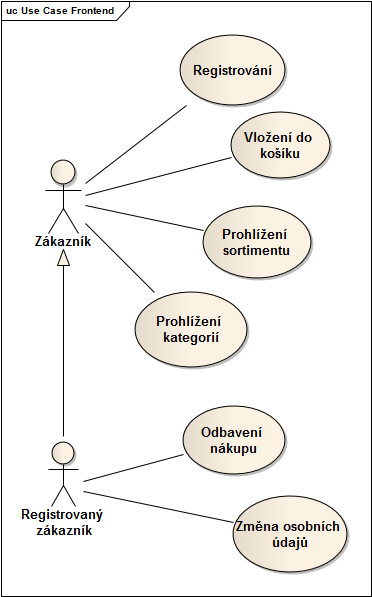
\includegraphics[scale=0.75]{figures/usecasefront}
\caption{Use cases zákaznické části}
\label{fig:usecasefront}
\end{center}
\end{figure}

\begin{figure}[h!]
\begin{center}
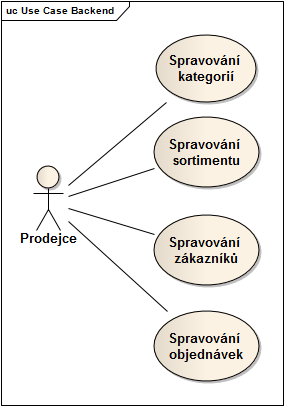
\includegraphics[scale=0.75]{figures/usecaseback}
\caption{Use cases administrační části}
\label{fig:usecaseback}
\end{center}
\end{figure}

\subsection{Scénář 1 - Prohlížení zboží v obchodu}
\subsubsection*{Role:}

\begin{itemize}
\item Neregistrovaný zákazník
\item Systém
\end{itemize}

\subsubsection*{Předpoklady:}

Zákazník se nachází na vstupní stránce internetového obchodu.

\subsubsection*{Důsledky:}

Zákazník získal informace, které hledal.

\subsubsection*{Hlavní příběh:}
\begin{enumerate}
\item Zákazník klikne na kategorii zboží.
\item Zákazník klikne na odkaz s názvem zboží, které ho zajímá.
\item Zákazníkovi se zobrazí informace o zboží.
\end{enumerate}

\subsubsection*{Možná rozšíření:}

\begin{description}
\item 1.1 Zákazník vyhledá zboží pomocí hledání
\item 2.1 Zákazník vyfiltruje zboží pomocí parametrů
\item 3.1 Zákazník klikne na odkaz \uv{Koupit} a tím vloží zboží do košíku.
\end{description}


\subsection{Scénář 2 - Registrace zákazníka}

\subsubsection*{Role:}

\begin{itemize}
\item Neregistrovaný zákazník
\item Systém
\end{itemize}

\subsubsection*{Předpoklady:}

Zákazník není přihlášený.

\subsubsection*{Důsledky:}

Zákazník je registrovaný v systému.

\subsubsection*{Hlavní příběh:}

\begin{enumerate}
\item Zákazník klikne na odkaz \uv{Registrovat}.
\item Zákazník vyplní osobní údaje.
\item Zákazník potvrdí registrační údaje.
\end{enumerate}

\subsubsection*{Rozšíření:}

\begin{description}
\item 3.1 Zákazník se odhlásí kliknutím na odkaz \uv{Odhlásit}.
\end{description}

\subsection{Scénář 3 - Nákup zboží}

\subsubsection*{Role:}

\begin{itemize}
\item Neregistrovaný zákazník
\item Systém
\item Správce obchodu
\end{itemize}

\subsubsection*{Předpoklady:}

Zákazník je přihlášený a nachází se na stránce produktu.


\subsubsection*{Důsledky:}

Zákazník má potvrzeno, že je zboží objednané.

\subsubsection*{Hlavní příběh:}

\begin{enumerate}
\item Zákazník klikne na odkaz \uv{Koupit} a vloží tak zboží do košíku.
\item Zákazník zkontroluje obsah košíku a klikne na odkaz \uv{Objednat}.
\item Zákazník vyplní údaje a zvolí způsob dopravy a platby.
\item Zákazník zkontroluje údaje a odešle je kliknutím na tlačítko \uv{Potvrdit}.
\item Zákazník dostane potvrzení od systému, že objednávka byla přijata.
\end{enumerate}

\subsubsection*{Rozšíření:}

\begin{description}
\item 1.1 Zákazník vloží do košíku další zboží.
\item 2.1 Zákazník si přečte obchodní podmínky pod odkazem \uv{Obchodní podmínky}.
\item 5.1 Správce obchodu kontaktuje zákazníka v případě komplikací s objednávkou.
\end{description}

\subsection{Scénář 4 - Přihlášení obchodníka}

\subsubsection*{Role:}

\begin{itemize}
\item Nepřihlášený správce
\item Systém
\end{itemize}

\subsubsection*{Předpoklady:}

Správce se chce přihlásit do administrace a zná administrační přihlašovací jméno a heslo. Nachází se na úvodní stránce aplikace.

\subsubsection*{Důsledky:}

Správce je přihlášený a může spravovat administraci.


\subsubsection*{Hlavní příběh:}

\begin{enumerate}
\item Správce klikne na odkaz \uv{Přihlásit}.
\item Správce zadá přihlašovací údaje do načteného formuláře a potvrdí jej.
\item Správce klikne na odkaz \uv{Administrace}.
\end{enumerate}

\subsubsection*{Rozšíření:}

\begin{description}
\item 3.1 Správce se odhlásí kliknutím na odkaz \uv{Odhlásit}.
\end{description}

\subsection{Scénář 5 - Vložení kategorie}

\subsubsection*{Role:}

\begin{itemize}
\item Přihlášený správce
\item Systém
\end{itemize}

\subsubsection*{Předpoklady:}

Správce je přihlášený a nachází se na hlavní stránce administrace.

\subsubsection*{Důsledky:}

V katalogu je nová kategorie.

\subsubsection*{Hlavní příběh:}

\begin{enumerate}
\item Správce klikne na odkaz \uv{Katalog}.
\item Správce klikne na odkaz \uv{Vložit kategorii}.
\item Správce vyplní informace o nové kategorii a zvolí nadřazenou kategorii.
\item Správce potvrdí informace kliknutí na tlačítko \uv{Vložit}.
\end{enumerate}

\subsubsection*{Rozšíření:}

\begin{description}
\item  4.1 Správce si zobrazí kategorii v katalogu.
\end{description}

\subsection{Scénář 6 - Vložení zboží}

\subsubsection*{Role:}

\begin{itemize}
\item Přihlášený správce
\item Systém
\end{itemize}

\subsubsection*{Předpoklady:}

Správce je přihlášený a nachází se na hlavní stránce administrace.

\subsubsection*{Důsledky:}

V katalogu je nové zboží.

\subsubsection*{Hlavní příběh:}

\begin{enumerate}
\item Správce klikne na odkaz \uv{Produkty}.
\item Správce klikne na odkaz \uv{Vložit produkt}.
\item Správce vyplní informace o novém zboží a zvolí nadřazenou kategorii.
\item Správce potvrdí informace kliknutí na tlačítko \uv{Vložit}.
\end{enumerate}

\subsubsection*{Rozšíření:}

\begin{description}
\item  3.1 Klikem s podrženou klávesou CTRL může zvolit správce více kategorií.
\end{description}

\section{Datový model}

Z důvodu uchování informací o zboží, o zákaznících, o objednávkách a dalších; je třeba zavést základní datový model, který se bude moci dále rozšiřovat.

Na Obrázku \ref{fig:datamodel} jsou znázorněné důležité entity propojené vazbami mezi sebou. Diagram pochází z aplikace Visual Studio, ve které byl e-shop kompletně naprogramován včetně návrhu datového modelu, viz. \ref{implprost}. Z diagramu vyplývá, že datový model je pouze minimální. Základní entity jako je  \texttt{BasicProduct} (zboží) a \texttt{BasicCategory} (kategorie) obsahují minimum vlastností pro reprezentaci v e-shopu. Kategorie je organizována ve stromové struktuře katalogu. Zboží je obsaženo v kategoriích a volitelně může být obsaženo ve více kategoriích.
	
Zboží se při nákupu ukládá uživateli do košíku \texttt{CartItem} s informacemi o množství a datumu. Při vytvoření objednávky se položky z košíku přesunou do detailu objednávky \texttt{OrderDetail} a ty se pak agregují do samotné entity objednávky \texttt{Order} spolu s informacemi o zákazníkovi. Volitelně, pokud je zákazník přihlášený se objednávka přiřadí k přihlášenému zákazníkovi \texttt{Customer}. 
	
Poslední důležité entity jsou zdroje \texttt{Resource} obsahující překlady do více jazyků a nastavení \texttt{Setting}, které uchovává obecná nastavení aplikace e-shopu.

	Samozřejmostí je možnost tento základní datový model rozšířit pomocí modulů. Toto je detailně probíráno v Kapitole \ref{sec:realizace}.
	
\begin{figure}[h!]
\begin{center}
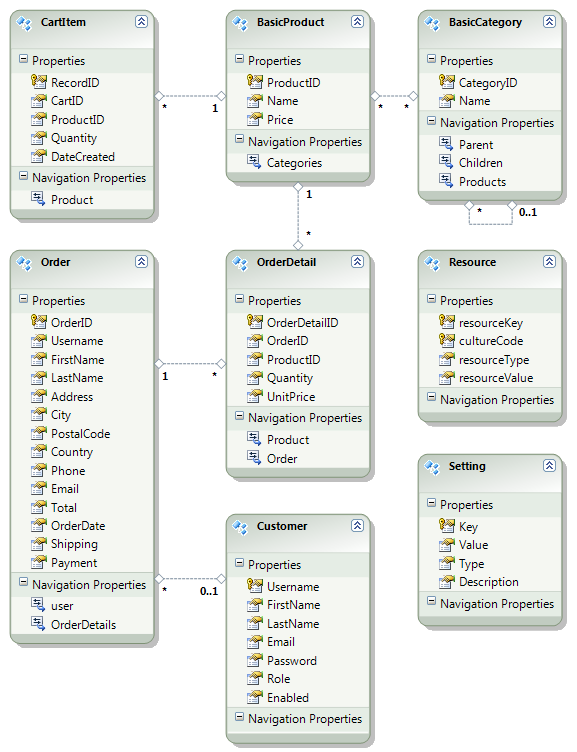
\includegraphics[scale=1]{figures/datamodel}
\caption{Základní datový model}
\label{fig:datamodel}
\end{center}
\end{figure}


\section{Návrhové vzory}

Pro rozsáhlou aplikaci navrženou v objektově orientovaném programovacím jazyce jsou návrhové vzory nutností. Neustále se opakující problémy při návrhu složitých aplikací jako je tato vyžadují analýzu všech známých návrhových vzorů. V následujících sekcích si představíme všechny vhodné vzory a probereme jejich klady, zápory a důvody, proč byly či nebyly vybrány. Všechny vzory jsou čerpány z literatury \cite{GOF} a \cite{PEAA}.

\subsection{Factory method}
Tento návrhový vzor se uplatní při vytváření instancí různých implementací rozhraní. Patří mezi vytvářecí návrhové vzory. Jeho využití je probíráno už v dalším vzoru \textit{Plugin}. Využití vzoru \textit{Factory method} spočívá v tom, že volaná metoda je továrnou na instance, které nemusí být ve třídě specifikované, ale využívají se pouze jejich předpisy v podobě rozhraní nebo abstraktních tříd. To přináší do kódu flexibilitu. Samotná metoda také nemusí být specifikovaná, její konkrétní podobu jí mohou dát až zdědění potomci.
Další volitelnou funkčností této metody může být inicializace až na žádost v době, kdy je instance třídy potřeba.

Diagram tříd \ref{fig:factorymethod} z \cite{GOF} popisuje způsob tvorby konkrétních instancí ve \textit{factory method}. Třída \texttt{Konkrétní tvůrce} již obsahuje tělo metody \texttt{factory method}, která vytváří třídu \texttt{Konkrétní Produkt}. Ten implementuje rozhraní \texttt{Produkt}, jehož předpis zná třída \texttt{Tvůrce} a v metodě \texttt{operace} s ním pracuje. Samozřejmě ve finále tuto metodu spouští až třída \texttt{Konkrétní Tvůrce}, pro zjednodušení v diagramu metoda uvedena podruhé není.

\begin{figure}[h!]
\begin{center}
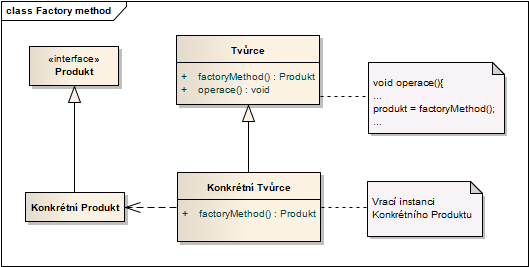
\includegraphics[scale=0.7]{figures/factorymethod}
\caption{Diagram tříd návrhového vzoru Factory method}
\label{fig:factorymethod}
\end{center}
\end{figure}


\subsection{Plugin}
David Rice a Matt Foemmel popisují návrhový vzor \textit{pluginu} jako vhodný prostředek pro odstínění různých implementací rozhraní. Pluginy se dají měnit za jiné přímo za běhu aplikace, bez potřeby překompilovávat aplikaci. Výměnu pluginu za jiný indikuje \textit{konfigurace}. Návrhový vzor plugin je v tomto případě velice jednoduchý a zakládá se na vytvoření instance z jedné implementace rozhraní. Volání implementovaných členů rozhraní se provádí po vytvoření instance implementace rozhraní například pomocí vzoru \textit{Factory method}. Toto popisuje sekvenční diagram z \cite{PEAA} - viz Obrázek \ref{fig:pluginseq}. Na tomto přístupu injektáže implementací rozhraní lze založit základy modulů v aplikaci e-shopu, viz dále.

\begin{figure}[h!]
\begin{center}
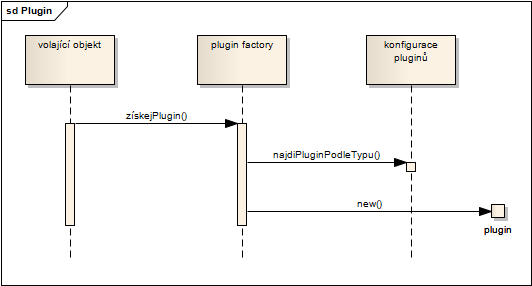
\includegraphics[scale=0.7]{figures/pluginseq}
\caption{Sekvenční diagram vytvoření pluginu}
\label{fig:pluginseq}
\end{center}
\end{figure}

Způsob konfigurace se liší implementaci od implementace, ale jednoduchou formou konfigurace je textový soubor XML s tagy označujícími konkrétní plugin, třeba formou cesty v souborovém systému ke zkompilované dynamické knihovně. Další formou konfigurace může být konvence, podle které se budou platné pluginy nacházet v určitém adresáři aplikace.

\subsection{Unit of Work}
Tento návrhový vzor se hodí na udržování seznamu datových objektů, které byly změněny aplikací a vyřizuje jejich správné zapsání do databáze a zároveň řeší konflikty při paralelních přístupech. Vzor se pro aplikaci hodí vzhledem k objemu předpokládaných transakcí s databází. Zvolená ORM vrstva \textsf{Entity Framework} ho již má implementovaný.

Diagram \ref{fig:uow} popisuje registraci změněného objektu v Unit of Work. Tuto registraci musí uživatel při změně objektu provédst sám. Toto to je volitelné proto, aby objekt Unit of Work nemusel zbytečně zapisovat všechny změny, které se do databáze promítnout nemusí. Objekt Unit of Work takto registruje všechny nové, změněné nebo smazané objekty pro pozdější promítnutí do databáze.
\begin{figure}[h!]
\begin{center}
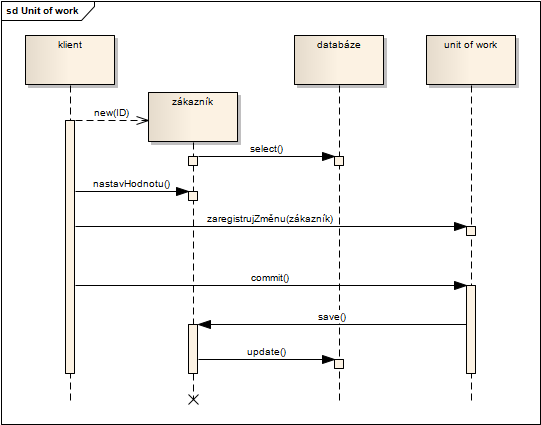
\includegraphics[scale=0.7]{figures/uow}
\caption{Sekvenční diagram registrace změněného objektu v Unit of Work}
\label{fig:uow}
\end{center}
\end{figure}


\subsection{Repository}

Jedná se o další návrhový vzor pro odstínění přístupu k databázi. Jeho předností je, že umožní plně objektově orientovaný způsob dotazování a všechno spojené s dotazy na databázi zapouzdřuje v sobě. Různé datové zdroje tak můžou být odstíněny za vrstvou potřebného počtu \textit{repositories}. Programátor používající \textit{repository} se tak může plně soustředit na práci s objekty, které potřebuje. Další výhodou je, že je konkrétní \textit{repository} vyměnitelné za jiné, které poskytuje jiná data nebo nepřistupuje k databázi. Toto je vhodné pro unit testy. Urychlí se tak běh testů. Zároveň je to perfektní příprava pro \textit{Dependency Injection}, které představíme dále. Další informace lze nalézt v \citep{PEAA}.

Vzor Repository nebyl do aplikace implementován, protože by vytvářel další vrstvu, kterou zastupuje Entity Framework s implementací vzoru Unit of work.

\subsection{Inversion of Control}

V současnosti velmi používaná metoda pro ovládání aplikace, která řeší řízení aplikace z jednoho místa. Článek Martina Fowlera celou  problematiku výstižně popisuje \cite{injection}. Toto je stručný extrakt z článku, kde je celá problematika \textit{Inversion of Control} probírána detailněji. Zabývá se v něm také rozdíly mezi souvisejícími návrhovými vzory \textit{Dependency Injection} a \textit{Service Locator}.

\textit{Inversion of Control} neboli česky \textit{převrácení ovládání}, je často používaný mechanismus ve frameworcích, které řídí program svojí hlavní programovou smyčkou a programátor se jen stará o doplňování funkcí a specifikací abstraktních tříd. Dříve bylo zvykem mít v programu vlastní hlavní ovládací smyčku. Pod pojmem \textit{Inversion of Control} se dá představit spousta věcí a spousta z nich bude správná, proto byly zavedeny již zmíněné úzce zaměřené vzory \textit{Dependency Injection} a \textit{Service Locator}, které si nyní ve stručnosti představíme.

\subsubsection{Dependency Injection}
Tento návrhový vzor spočívá ve vkládání závislostí - konkrétních rozhraní - do tříd pomocí řídící třídy, která zná všechny potřebné informace. Řídící třída se většinou nazývá \uv{kontejner}. Obrázek \ref{fig:di} vzor názorně ilustruje. Separátní objekt \texttt{Kontejner} obsadí proměnnou ve třídě \texttt{Výpis} s vhodnou implementací rozhraní \texttt{Vyhledávání}.

\begin{figure}[h!]
\begin{center}
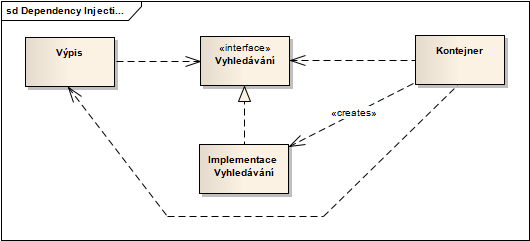
\includegraphics[scale=0.75]{figures/di}
\caption{Závislosti ve vzoru Dependency Injection}
\label{fig:di}
\end{center}
\end{figure}


Metody, jak dostat závislá rozhraní do třídy, jsou tři.

\begin{itemize}
\item \textbf{Constructor injection} -- parametr v konstruktoru při vytváření instance třídy slouží jako prostor pro Dependency Injection. Nevýhoda je, že závislost lze vyřešit jen při vytváření instance na počátku. Výhodou je, že třída má zaručeno naplnění závislosti.
\item \textbf{Setter injection} -- vyřešení závislosti pomocí setteru. Výhoda je, že se kvůli závislosti nemusí měnit konstruktor třídy. Nevýhoda je zřejmá. Je nutné dávat pozor na včasné naplnění závislosti. To se bohužel nepozná při sestavování, ale až při běhu.
\item \textbf{Interface injection} -- tato metoda není tak obvyklá a spočívá v implementaci injekčních rozhraní obsahujících potřebné informace. Další vlastnosti a detaily této metody jsou uvedeny v článku \cite{injection}.
\end{itemize}

Pro tento návrhový vzor existují hotová řešení pro každý objektově orientovaný jazyk v podobě IoC Containerů.

\subsubsection{Service Locator}

Další velmi podobný vzor pro řešení závislostí. Jeho nevýhodou je složitější způsob testování unit testy. Následující obrázek \ref{fig:servicelocator} popisuje způsob chování.

\begin{figure}[h!]
\begin{center}
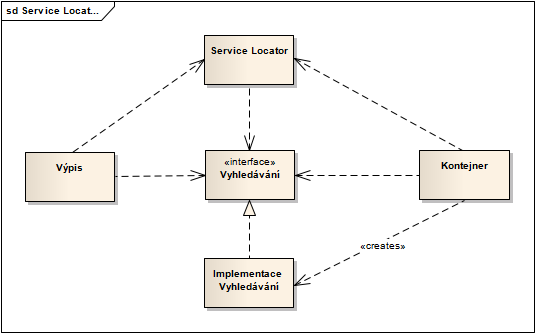
\includegraphics[scale=0.75]{figures/servicelocator}
\caption{Závislosti ve vzoru Service Locator}
\label{fig:servicelocator}
\end{center}
\end{figure}

Z diagramu vyplývá podobně jako u vzoru \textit{Dependency Injection}, že má opět vzor objekt \texttt{Service Locator}, který se stará o vyhledávání služeb vyžadovaných ve třídě \texttt{Výpis} a voláním určité metody dodá třídě \texttt{Výpis} implementaci \texttt{Implementace Vyhledávání}. Samozřejmě je třeba opět vyřešit závislost při dodávání \texttt{Service Locator} do \texttt{Výpis}u. 

Od vzoru \textit{Service Locator} se v poslední době ustupuje vzhledem k požadavkům na testovatelnost aplikací pomocí unit testů, které se píší o něco složitěji než pro vzor \textit{Dependency Injection}. 




\section{Architektura}
Požadavky na architekturu jsou vzhledem k rozsáhlosti aplikace a její komplikovanosti velmi specifické. Jedná se o webovou aplikaci a tedy můžeme vybrat jako základ některý ze známých architektonických vzorů. 

\begin{samepage}
Webové architektury se vytvářejí nejčastěji jako 2 nebo 3 úrovňové. Aplikace je tak rozdělena do částí starajících se o 

\begin{enumerate}
\item Zpracování požadavků uživatele
\item Práci s daty v aplikaci
\item Prezentaci výstupu uživateli
\end{enumerate}
\end{samepage}

Dvouúrovňová architektura je pouze spojením některých dvou z výše zmíněných částí. O celku nerozlišujícím mezi těmito částmi nelze pak mluvit o architektuře, ale jde o amatérský počin bez smysluplného uspořádání, kterým si většina z programátorů webových aplikací zajisté sama prošla.

Jako nejznámější architektonický vzor využívající všech tří vrstev je dlouho známý vzor Model View Controller. Nemá cenu rozebírat jiné vzory, protože jsou to varianty na tento vzor.

\subsection{Model View Controller (MVC)}
\label{mvc}
Vzor je známý již ze 70. let minulého století, kdy s ním jako první oficiálně přišel Trygve Reenskaug jako s frameworkem pro SmallTalk. Od té doby sehrál významnou roli v návrhu frameworků a aplikací s uživatelskými rozhraními\citep{PEAA}. Základní princip popisuje velmi jednoduchý diagram \ref{fig:mvc}.

\begin{figure}[h!]
\begin{center}
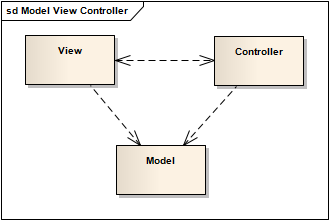
\includegraphics[scale=0.75]{figures/mvc}
\caption{Model View Controller}
\label{fig:mvc}
\end{center}
\end{figure}

V této architektuře jsou důležité již dříve zmiňované prvky, tentokráte s konkrétními pojmenováními.

\begin{description}
\item[Model] se v aplikaci stará o poskytování a změnu dat, ať už z databáze nebo z jiných zdrojů. Jde o objekt představující čistě data bez jakýchkoli vizuálních prvků.
\item[View] (\textit{pohled}) se stará o zobrazení modelu pomocí vizuálních prvků uživateli. Využívá k tomu technologie HTML a dalších doplňků. Data nemá možnost měnit.
\item[Controller] (\textit{řídící část}) se stará o zpracování požadavků přicházejících od uživatele. Po zpracování požadavku změní \textit{model} a nastaví správné zobrazení \textit{pohled}u.
\end{description}

Další podrobnější informace lze najít v \citep{PEAA}. Vzor MVC je implementován v různých frameworcích třetích stran u většiny zmíněných programovacích platforem v sekci \ref{sec:reserse}.

\subsection{Modularita v Model View Controller}

Z pohledu požadavků na aplikaci modulárního e-shopu je nutné uvažovat o vhodné rozšiřitelnosti architektonického vzoru MVC. Nabízí se několik možností:

\begin{enumerate}
\item Rozšíření o další Controllery, které budou ovládat rozšiřující funkce. Tato možnost je samozřejmá ve všech frameworcích podporujících MVC. Controllery jsou věnované vždy několika společným funkcím. Například Controller pro zboží, zákazníky, objednávky, přihlašování, atd. V tomto případě využívají Controllery vlastní Pohledy. Modely mohou používat buď společné nebo opět vlastní. V případě kompilačních jazyků se musí vždy aplikace znovu sestavit a spustit, což je nevýhoda.

\item Rozšíření o skupiny Controllerů. Ve frameworcích se těmto skupinám říká \textit{oblasti} (\texttt{Areas}) nebo \textit{moduly} (\texttt{Modules}). Nejedná se přímo o připravené moduly fungující ihned po připojení k aplikaci. U kompilačních jazyků se musí opět aplikace sestavit a spustit. Rozšiřující oblasti jsou v souborovém systému rozděleny podle adresářů nebo jmenných prostorů (\texttt{namespaces}) a často se jedná o oddělení aplikačních částí frontendu a backendu. V prostředí .NET ve frameworku MVC existují rozšíření, která fungují na tomto principu rozšíření. Jedním je například Portable Areas \footnote{\url{http://portableareas.codeplex.com/}}, projekt se ale dále již nerozvíjí.

\item Rozšíření o externí balíčky obsahující kompletní rozšiřující funkce včetně Controllerů, Pohledů i Modelů. Jde o nejpokročilejší možnost ze zmiňovaných. Vlastnosti předchozích možností jsou využity i zde. Jde ale o způsob nahrávání a integrace těchto funkcí do již hotového řešení. Aplikaci je třeba navrhnout tak, aby poskytovala body pro rozšíření i mimo předchozí možnost seskupování Controllerů. V této variantě jdou rozšířit i další části hotové aplikace včetně Modelů a Pohledů. Nevýhoda tohoto řešení je složitost. Výhoda je, že se hotová aplikace nemusí znovu sestavovat, stačí dodat jen sestavené moduly a aplikaci spustit.
\end{enumerate}


Implementace modulární architektury si vyžádala nejsložitější řešení vzhledem k požadavkům na aplikaci e-shopu. Specifiky tohoto řešení se zabývá kapitola Implementace \ref{sec:realizace}.


\section{Implementační prostředí}
\label{implprost}
Zvoleným prostředím byla po provedení  Rešerše v kapitole \ref{sec:reserse} zvolena platforma Microsoft .NET. Zvolil jsem tuto platformu z několika důvodů:

\begin{itemize}
\item Platforma .NET je navržena a udržována velkou softwarovou společností.
\item Platforma má velké množství uživatelů.
\item Platforma je celistvá a poskytuje vlastní kvalitní IDE - Visual Studio.
\item Pracovní nástroje platformy jsou dostupné zdarma.
\item Existují hostingy i nabídky dedikovaných serverů pro tuto platformu.
\item Platforma se rychle vyvíjí.
\item Pro platformu je dostupný framework pro webové aplikace s architekturou MVC v dostatečně odladěné a rozšiřitelné verzi.
\item Použitý programovací jazyk C\# je podobný jazyku Java, se kterým jsem již pracoval.
\item Na této platformě existuje spousta rozšiřujících knihoven ulehčujících práci.
\item Na této platformě jsem nikdy neprogramoval webové aplikace, a proto je pro mě tato volba i výzvou.
\end{itemize}


\subsection{Rozšiřující knihovny pro platformu .NET}
\label{subsec:roz}
V této části budou probrány zajímavé knihovny platformy Microsoft.NET použité v této práci. Některé z těchto knihoven jsou lehce integrovatelné do projektů pomocí speciálního balíčkovacího systému \textbf{NuGet}\footnote{\url{http://nuget.org/}}, který je dostupný jako rozšíření pro Visual Studio. \textit{NuGet} poskytuje rozšíření, která se snadno instalují jedním kliknutím a sám se postará o jejich nastavení. Rozšíření pro systém \textit{NuGet} jsou poskytovány jak nezávislými vývojáři, tak přímo od Microsoftu. Knihovnu pro \textit{NuGet} může napsat každý snadno a rychle.

\subsubsection{ASP.NET MVC 3}
V první řadě je třeba zmínit hlavní knihovnu, na které je jádro aplikace postavené a tou je framework ASP.NET MVC 3. Něco málo o něm bylo řečeno už v kapitole Rešerše \ref{asp.net} a o jeho architektuře v předchozí sekci \ref{mvc}. Všechny jeho vlastnosti jsou detailně popsány na webových stránkách frameworku\footnote{\url{http://www.asp.net/mvc}} pomocí skvělých videí a textových tutoriálech.
 
\subsubsection{Entity Framework - Code First}
\label{sec:ef}
Microsoft přišel před několika lety s novým ORM frameworkem, který se stal soupeřem NHibernate. V poslední verzi 4 už je Entity Framework\footnote{\url{http://msdn.com/data/ef}} na použitelné úrovni. Entity Framework nabízí 3 různé způsoby, jak založit databázové úložiště. 

\begin{itemize}
\item Jedním způsobem je \textit{Code First}. Spočívá v nulovém návrhu databáze. Proto se mu říká \textit{Code First} (\textit{nejdříve kód}). Nejprve se navrhnou entity ve formě tříd a jejich vztahy se navážou přes otypované parametry. Jakákoli změna entit je detekována a databáze se podle pravidel přeorganizuje. V další verzi 4.2 se představí vlastnost zvaná \textit{Migrations}, která dokáže opravit změny v databázi bez nutnosti přehrávání celé databáze, což byla velice kritizovaná vlastnost. Musela se řešit zálohováním dat nebo zapsáním pevných iniciálních dat do kódu. Jinak se Microsoft snaží tento způsob návrhu databáze upřednostňovat ve všech svých tutoriálech.

\item Další způsob je \textit{Model First}. Jde o způsob, jenž předpokládá, že má programátor již hotový model databáze ve formátu vhodném pro Entity Framework. Z modelu se vygenerují třídy zastupující entity a dále se pokračuje jako při prvním způsobu. 

\item Poslední třetí způsob je \textit{Database First}. Tento případ předpokládá, že programátor má přístup k již existující databázi. Z ní se potom vygenerují opět entity.

\end{itemize}

Model, přes který se převádí databáze na entity a naopak se jmenuje \textit{Entity Data Model} (EDM) a staví na známém ER modelu od Dr. Petera Chena. K dotazování na databázi se využívá jazyka LINQ, který poskytuje nápovědu při psaní kódu a kontrolu syntaxe během kompilace. Entity Framework je postavený nad ADO.NET provider modelem a proto jsou přes něj dostupné všechny funkce. Díky tomu se také může aplikace připojit na různé databáze od MS SQL přes DB2 po Oracle\cite{efintro}.


\subsubsection{SQL Compact Edition}
Nejedná se o knihovnu, ale o databázi a je třeba o ní ztratit pár slov, protože byla použita v aplikaci. Je to nejmenší verze z nabízených databází Microsoftu a je přednastavená při vytváření základní šablony aplikace ve frameworku MVC 3 ve Visual Studiu. V projektu jde o verzi SQL Server Compact Edition 4.

Jde o databázi uloženou v jednom souboru společně s aplikací, její možnosti jsou omezené. Nevýhodou je, že nejde profilovat dotazy do databáze pomocí profesionálních databázových nástrojů jako je SQL Server Management Studio. Na druhou stranu je zdarma a obsahuje kompaktní databázový systém přímo v jednom souboru, takže není třeba databázový systém instalovat. Microsoft bohužel nenabízí srovnání s ostatními verzemi, ale našel jsem dokument, který se tímto zabývá \footnote{\url{http://coolthingoftheday.blogspot.com/2011/01/sql-server-compact-4-vs-sql-server.html}}. Srovnání a další dostupné verze (mezi nimiž je třeba zmínit edici Express, která je zdarma) jsou dostupné online na webových stránkách MS SQL Serveru\footnote{\url{http://www.microsoft.com/sqlserver/en/us/product-info/compare.aspx}}.


\subsubsection{Castle Windsor}
Tato knihovna je jedním z mnoha \textit{Inversion of Control kontejnerů} pro ASP.NET framework. Byla vybrána z důvodu potřeby použít IoC kvůli načítání funkcí z modulů. Pro Castle Windsor hovoří dobrá dokumentace\footnote{\url{http://stw.castleproject.org/Windsor.MainPage.ashx}} a množství možností. Důležitá je možnost načítat implementace rozhraní pomocí reflexe ze \textit{sestavení} (\textit{assemblies}). Funguje na principu vzoru \textit{Dependency Injection}. Nejprve se vytvoří \texttt{Container}, do něho se registrují rozhraní a jejich implementace. Poté se závislosti při běhu programu řeší na požádání.

\subsubsection{Paged List}
Pro stránkování byla využita knihovna \textit{Paged List}\footnote{\url{https://github.com/TroyGoode/PagedList}}. Její předností je usnadněná práce při vytváření odstránkovaných seznamů. Dále nabízí možnosti nastavení vzhledu stránkovacích odkazů na pohyb mezi stránkami.

\subsubsection{Glimpse}
\label{glimpse}
Tato vynikající knihovna\footnote{\url{http://getglimpse.com/}} je takový doktor na všechno. Je to diagnostický nástroj zabudovaný přímo do aplikace. Načte se na požádání s rozhraním webové aplikace jako další okno a obsahuje důležité informace, které debugger Visual Studia nezná. Díky němu se dají aplikace napsané v MVC frameworku ladit jednoduše a rychle. Knihovna zamezí spoustu problémům a ušetří pár zničených klávesnic a monitorů u více vznětlivých webových vývojářů.

\subsection{Ostatní použité technologie}
Ještě stojí krátce za zmínku použité technologie na straně uživatelského rozhraní, které jsou standardně použité už v šabloně projektu MVC frameworku ve Visual Studiu.

\subsubsection*{HTML 5}
HTML 5 je novou verzí dlouho ctěného standardu HTML 4, který je pro potřeby moderního webu již zastaralý. 5. verze přináší nové tagy pro audio, video a grafiku. Dále se zaměřuje na vylepšení sémantického významu částí stránky pomocí dalších tagů jako je section, article, header a nav. Další změny jsou ve formulářových polích, které by měly podporovat nové způsoby vkládání a nové datové typy. Další je podpora ukládání dat na straně uživatele a jejich zachovávání\footnote{\url{http://en.wikipedia.org/wiki/HTML5}}. HTML 5 bude muset urazit ještě dlouhou cestu standardizačními procesy, než se stane obecně standardem. Naštěstí se Microsoft vzpamatoval a poslední verze Internet Exploreru už nestandardizované HTML 5 podporuje.

\subsubsection*{CSS 3}
Další verze kaskádových stylů na formátování vzhledu HTML dokumentů. Ve verzi 3 ještě nejsou také standardizované, ale prohlížeče je částečně podporují, nebo lze využít vlastních tagů prohlížečů. Poslední verze nabízí vychytávky jako víceobrázková pozadí, přechody, transparentnost, více-sloupcový layout, média, atd. Bohužel si ještě nějaký rok budeme muset na finální standard počkat.

\subsubsection*{Javascript a JQuery}
Javascript\footnote{\url{http://cs.wikipedia.org/wiki/JavaScript}} tu s námi je už od roku 1997, kdy byl standardizován asociací ECMA. Jde o netypový objektový skriptovací jazyk používaný pro manipulaci se vzhledem a daty na straně uživatele. Přestože je velmi náchylný k chybám, zažil boom s nástupem AJAXu a frameworků jako je \textit{JQuery}\footnote{\url{http://jquery.com}}, které usnadňují skriptování a nabízejí přidané funkce. Díky JQuery bylo napsáno mnoho pluginů, které vylepšují přívětivost webů a usnadňují navigaci. V aplikaci e-shopu je například použit jako standardní validátor uživatelských formulářů JQuery plugin \textit{Validation}\footnote{\url{http://bassistance.de/jquery-plugins/jquery-plugin-validation/}}, který spolupracuje s ASP.NET MVC 3 frameworkem a předává si informace o formulářových políčkách a jejich obsahu.

Dokonce i javascriptové knihovny jako je \textit{JQuery} a její pluginy jsou vhodné pro distribuci pomocí balíčkovacího systému \textit{NuGet}, který je zmíněn v úvodu této sekce o Rozšíření \ref{subsec:roz}.

Ještě k doplnění, experimentální uživatelské rozhraní aplikace využívá také \textit{JQuery} pluginy \textit{JQuery UI}\footnote{\url{http://jqueryui.com/}}, \textit{Modernizr}\footnote{\url{http://www.modernizr.com/}} a \textit{JsTree}\footnote{\url{http://www.jstree.com/}}.




%*****************************************************************************
\chapter{Realizace}
\label{sec:realizace}

Tato kapitola se věnuje rozboru implementace e-shopu. Kromě popisu nestandardních postupů v implementaci také okrajově popisuje standardní způsoby realizace.

Znázornění struktury aplikace podle komponentů v balíčcích je zobrazeno v diagramu \ref{fig:components}. Popis částí komponent následuje v další sekci.

\section{Komponenty aplikace}
Z důvodu velké složitosti struktury aplikace je zde popsán diagram komponent, který graficky znázorňuje části aplikace v balíčcích a v nich obsažených komponentách, viz Obrázky \ref{fig:components} a \ref{fig:componentslow}.

První schéma \ref{fig:components} popisuje závislosti mezi sestavením frameworku, jádra a modulů. Všechny tyto části se napojují na Entity Framework pro získání dat z databáze pomocí dotazů v jazyku LINQ. Sestavení \textsf{Framework} obsahuje rozhraní služeb -- \textsf{Services}, datové entity -- \textsf{Entities}, jazykový překladač -- \textsf{Translator}, správu účtů -- \textsf{Account Management} a komponentu pro řešení závislostí -- \textsf{Dependency Injection}.

Na sestavení \textsf{Framework} závisí pak sestavení jádra -- \textsf{Core} a všechna sestavení modulů \textsf{Module}. Tyto sestavení pak mají další komponenty. Sestavení \textsf{Core} obsahuje kromě společných komponent s \textsf{Modul}y (\textsf{Frontend},\textsf{Backend}, \textsf{Routing}) navíc komponentu \textsf{Startup}, která se stará o inicializaci a spuštění aplikace a používá i funkce komponenty \textsf{Dependency Injection} v sestavení \textsf{Framework}, aby vyřešila závislosti při načítání komponent ze sestavení všech přidaných \textsf{Modulů} do základu aplikace.

\begin{figure}[h!]
\begin{center}
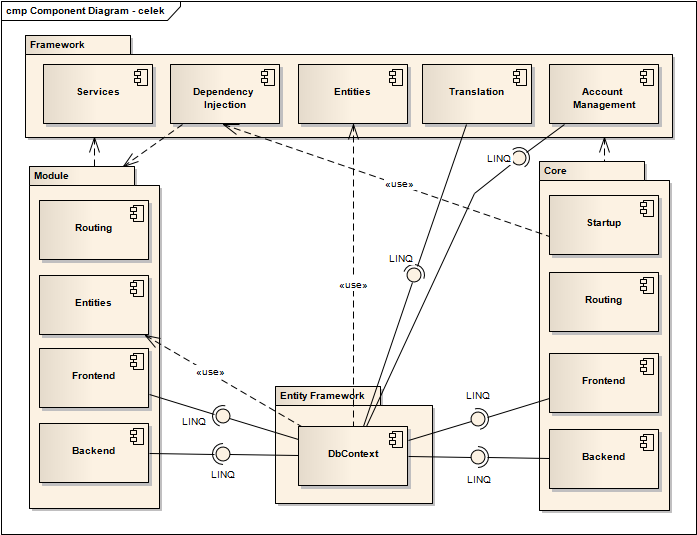
\includegraphics[scale=0.65,angle=0]{figures/componentsextract}
\caption{Diagram komponent}
\label{fig:components}
\end{center}
\end{figure}

\begin{figure}[h!]
\begin{center}
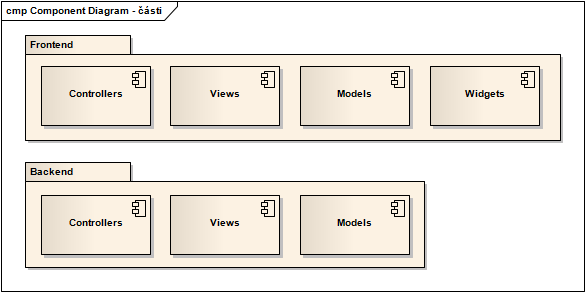
\includegraphics[scale=0.75,angle=0]{figures/componentslow}
\caption{Diagram komponent -- část nižší úrovně}
\label{fig:componentslow}
\end{center}
\end{figure}

Obrázek \ref{fig:components} obsahuje pouze nejdůležitější vazby mezi sestaveními a komponentami. Je to z důvodu přehlednosti. Další obrázek \ref{fig:componentslow} zobrazuje vnořené komponenty v balíčcích \textsf{Frontend} a \textsf{Backend}. Balíčky jsou v diagramu \ref{fig:components} zobrazeny jako komponenty v sestavení \textsf{Core} a \textsf{Module}. Obsahují standardní komponenty MVC architektury, které jsou v balíčku \textsf{Frontend} doplněné o komponentu \textsf{Widgets}. Tu si probereme v sekci \ref{sec:widgets}.





\section{Použité části ASP.NET MVC 3}

V této části si probereme základní použité části frameworku ASP.NET MVC 3, které byly využity v aplikaci. Tyto části zde zmíníme do hloubky nutné k pochopení dalšího popisu aplikace. Doporučuji však pro bližší seznámení s frameworkem také tutoriály \footnote{\url{http://www.asp.net/mvc/tutorials}} a knihy \cite{MVC1} a \cite{MVC2}. 

\begin{figure}[h!]
\begin{center}
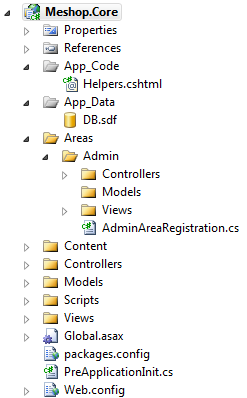
\includegraphics[scale=0.99]{figures/struktura}
\caption{Základní struktura projektu}
\label{fig:struktura}
\end{center}
\end{figure}

Pro přehlednost stojí za zmínku základní adresářová struktura projektu používající framework MVC 3, viz. Obrázek \ref{fig:struktura}. Povinné v ní není prakticky nic, ale pokud bychom se rozhodli strukturu nedodržet, musíme přinejmenším upravit cesty pro \textsf{Views} specifikací \texttt{RazorViewEngine}, o tom dále v \ref{sec:views}. \textsf{Properties} obsahují konfiguraci projektu. \textsf{References} je pseudoadresář pro zobrazení načtených potřebných dynamických knihoven. 

V adresářích s předponou \textsf{App\_} jsou zdroje používané pro databázové soubory, textové prostředky -- \textsf{resources} a sdílené třídy. Adresář \textsf{Areas} obsahuje \textit{oblasti} oddělené od sdílených tříd v projektu pomocí \textsf{namespace}. Adresáře \textsf{Content} a \textsf{Scripts} obsahují soubory pro zobrazení a client-side skripty. 

Ostatní adresáře jsou jasné podle jejich pojmenování a obsahují třídy a prvky popsané níže. Soubor \textsf{Global.asax} je startovním souborem zastupující modul \textsf{Startup}. 

Nepovinný soubor \textsf{PreApplicationInit.cs} obsahuje prvky pro inicializaci sestavení modulů při startu aplikace. Soubor \textsf{Web.config} je XML konfigurace aplikace, kterou používá IIS web server. \textsf{Packages.config} je XML soubor pro systém \textit{NuGet} balíčků s výpisem instalovaných knihoven z \textit{Nuget} repozitáře.


\subsection{Global.asax}
Soubor \texttt{Global.asax} se spouští jako první při startu aplikace, proto je vhodné ho zmínit na začátku. Obsahují ho všechny aplikace v ASP.NET. Jako ukázka poslouží následující zhuštěný a ořezaný kód \ref{list:global.asax} přímo z aplikace. 

\begin{lstlisting}[float=h!,language=CSharp, caption={Global.asax}, label=list:global.asax]
public class MvcApplication : HttpApplication
{
    protected void Application_Start()
    {
        Framework.DI.Modules.Initialize();
        RegisterRoutes(RouteTable.Routes);          
        Framework.DI.Modules.RegisterAdapters();
        ControllerBuilder.Current.SetControllerFactory(
        						Framework.DI.Modules.GetControllerFactory());
        ViewEngines.Engines.Add(new MeshopViewEngine());
        //database refill
        Database.SetInitializer(new DatabaseInitializer()); 
    }
    protected void Application_End()
    {
        Framework.DI.Modules.Dispose();
    }
}
\end{lstlisting}

V metodě \texttt{Application\_start} se registrují jednotlivé části frameworku MVC a komponenty vlastního frameworku aplikace, které mění standardní funkčnost. Detaily jednotlivých částí jsou probrány v následujících podsekcích, v další sekci rozšíření \ref{sec:roz} a připojení modulů \ref{subsec:pripojenimodulu}. Po ukončení aplikace, což probíhá u webových aplikací zřídkakdy, se spustí metoda \texttt{Application\_End}, která v tomto případě zavolá metodu pro uvolnění registrovaných dat v IoC kontejneru z paměti.


\subsection{Controller}
Controller\footnote{\url{http://msdn.microsoft.com/en-us/library/system.web.mvc.controller.aspx}} je abstraktní třída, která poskytuje metody odpovídající na HTTP požadavky, viz. architektura \ref{mvc}. Specifikací této třídy implementujeme vlastní metody, které poskytují uživateli obsah z \textsf{Model}ů  pomocí pohledů -- \textsf{View}. 

V ukázce kódu \ref{list:controller} je vidět, jak se provádí specifikace. Metoda \texttt{Index} vrací výsledek \texttt{ActionResult} pomocí metody \texttt{View} s parametrem dat z modelu. Framework MVC zpracuje tento výsledek pomocí interních funkcí a odešle zpracovaný pohled. 

\begin{lstlisting}[float=h!,language=CSharp, caption={Controller}, label=list:controller]
public class HomeController : Controller {  
        public ActionResult Index()
        {
            var products = ProductModel.GetAll();
            return View(products);
        }
	//..dalsi metody ...        
}
\end{lstlisting}

\subsection{View}
\label{sec:views}
View neboli \textsf{Pohled} se používá pro zobrazení odpovědi aplikace uživateli, viz. architektura MVC \ref{mvc}. V případě frameworku MVC jde o několikavrstvého poskytovatele pohledů -- \texttt{RazorViewEngine}\footnote{\url{http://msdn.microsoft.com/en-us/library/system.web.mvc.razorviewengine.aspx}}. Jako obsah se používají soubory, které implicitně dědí od \texttt{WebViewPage}\footnote{\url{http://msdn.microsoft.com/en-us/library/system.web.mvc.webviewpage.aspx}}. Obsahem jsou šablony v šablonovacím jazyku \textsf{Razor}, který je rychlý a intuitivní pro vývojáře, kteří už nějaký šablonovací jazyk používali. Kód \ref{list:razor} poskytuje malou ukázku. 

\begin{lstlisting}[float,language=HTML, caption={Pohled s jazykem Razor}, label=list:razor]
@model IEnumerable<Meshop.Framework.Model.BasicCategory>
@{
    ViewBag.Title = "Categories";
}
<h2>@ViewBag.Title</h2>
<h3>@T("About")</h3>

@Html.ActionLink("Edit", "Edit", null, new { id = "edit" })

<div id="categories">
	<ul>
	@foreach (var item in Model) {
		<li>First</li>
    	@Helpers.RecurseBasicCategory(item,Html)          
	}
	</ul>
</div>
\end{lstlisting}

Jazyk \textsf{Razor} se vepisuje přímo do HTML tagů a kombinuje se s nimi. Ke slovu také přichází tzv. \texttt{Helpery}, které usnadňují psaní a generují kód ve spojení s HTML. Proces od napsání šablony po zobrazení je ve frameworku několikafázový. Nejprve se napíše pohled a propojí se s \texttt{Controllerem}, poté se aplikace zkompiluje, ale pohledy standardně zůstanou nezkompilované a nahrají se do ostrého prostředí ve struktuře shodné s vývojovou. Až teprve při požadavku na zobrazení pohledu se pohled dynamicky na požádání přeloží do C\# jazyka, zkompiluje se a je poslán jako odpověď přes HTTP k uživateli. 

Za zmínku stojí silně a dynamicky typované proměnné -- \textit{silně typovaný} \texttt{Model} a \textit{dynamický} \texttt{ViewBag}, které předávají data z akcí \texttt{Controlleru}. Systém pohledů také umožňuje sdílet \textsf{Layout} pro skupiny pohledů.

Pokud se vrátíme k ukázce \ref{list:razor}, můžeme si všimnout použití výše zmíněných prvků. Silně otypovaný model obsahující list entit na řádku \textbf{1}. Přepnutí do jazyka \textsf{Razor} pomocí \texttt{@} na řádku \textbf{2}. Použití dynamické sdílené proměnné \texttt{ViewBag} na řádku \textbf{3}. Ta je i následně na řádku \textbf{5} použita pro výpis. Na řádku \textbf{6} je použita vlastní implementace překládání textu, o které si řekneme více v sekci \ref{subsec:lokalizace}. Snad jen zmíním část implementace v pohledech. \texttt{T} je vlastní parametr ve vlastní verzi rodičovské třídy \texttt{WebViewPage} plněný singletonem \texttt{TranslationResolver}. Na řádku \textbf{8} je ukázka standardního helperu MVC. \textbf{12}. řádek pak ukazuje možnosti iterace v šablonách a kombinaci HTML s \textsf{Razor}. \textbf{14}. řádek je ukázka volání vlastního \texttt{Helperu}.

\subsection{Model}
Modely jsou ve frameworku MVC celkem komplikované, protože data reprezentují i sbírají od uživatelů z formulářů a přes Entity Framework (v tomto případě) je ukládají nebo načítají z databáze. Pro jejich úplné pochopení doporučuji prostudování kapitol 4,6 a 13 z knihy \cite{MVC1}.

Ve zkratce jsou modely sady entit pro práci se specifickými \textsf{pohledy} a nemusí  odpovídat tabulkám v databázi. Modelem může být entita nebo třída obsahující entity a parametry. V předchozí ukázce kódu \textsf{pohledu} \ref{list:razor} je modelem list entit, které se podle požadavků vypíší na obrazovku do formuláře nebo jako text. V následujícím kódu \ref{list:model} je ukázka modelu obsahující entity pro zobrazení v \textsf{Pohledu}. 

V další ukázce \ref{list:entita} je kód entity sloužící zároveň i jako model. Je zde zároveň vidět, jaké entita používá doplňkové \textsf{atributy} pro specifikaci názvu pole, který je možné přeložit -- atribut \texttt{TranslateName}. Dále jsou zde atributy pro upřesnění Entity Frameworku, jaké má  aplikovat omezení a klíče v DDL pro databázi. Více o atributech v sekci Validace dat \ref{sec:validacedat} a Atributy \ref{sec:atributy}.

\begin{lstlisting}[float=h!,language=CSharp, caption={Model z více entit}, label=list:model]
public class CategoryModel
{
	public BasicCategory Category { get; set; }
	public IEnumerable<BasicCategory> Categories { get; set; }
	public IEnumerable<BasicProduct> Products { get; set; } 
	
	public CategoryModel(BasicCategory c,IEnumerable<BasicProduct> p, IEnumerable<BasicCategory>  cs )
	{
		Categories = cs;
		Category = c;
		Products = p;
	}
}
\end{lstlisting}

\begin{lstlisting}[float=h!,language=CSharp, caption={Entita a zároveň Model}, label=list:entita]
public class BasicProduct
{
    [Key]
    [ScaffoldColumn(false)]
    public int ProductID { get; set; }

    [Required]
    [TranslateName("Name")]
    public string Name { get; set; }

    [Required]
    [TranslateName("Price")]
    public decimal Price { get; set; }

    [TranslateName("Categories")]
    public List<BasicCategory> Categories { get; set; }
}
\end{lstlisting}


\subsection{Routování}
\label{sec:routovani}

Routování je neoddělitelnou součástí všech moderních frameworků založených na architektuře MVC. Díky této další vlastnosti frameworku jsou adresy URL nasměrovatelné na metody v \texttt{Controllerech}. Díky tomu lze vytvářet různé aliasy a textové odkazy vhodné pro SEO i pro čitelnost člověkem. \texttt{Route}, nebo-li \textit{cesta} je uložena do datového slovníku a je dostupná obousměrně, pro generování odkazů v šablonách i pro rozpoznání metody v \texttt{controlleru} a parametrů podle URL. Z ukázky kódu \ref{list:route} lze snadno vyvodit způsob zápisu cesty. Routy jsou dostupné v aplikaci MVC přes singleton \texttt{RouteTable} a jeho metodu \texttt{Routes}.

\begin{lstlisting}[float=h!,language=CSharp, caption={Route}, label=list:route]
routes.MapRoute(
				"Default", // Route name
				"{controller}/{action}/{id}", // URL with parameters
				new { 
					controller = "Home", 
					action = "Index", 
					id = UrlParameter.Optional } // Parameter defaults
				);
\end{lstlisting}

Routy se registrují už při startu aplikace, proto je třeba inicializovat registraci v souboru \texttt{global.asax}, zmíněném na začátku sekce \ref{list:global.asax}.

\subsection{Areas}
\label{sec:areas}
Pomocí \textsf{Areas}, česky \textit{oblastí}, lze oddělit strukturálně komponenty aplikace. Slouží také pro udržení přehlednosti a zamezení konfliktů se stejnými názvy tříd, protože jsou v jiném \textit{namespace}. Jejich registrace se provádí pouze do komponenty \textsf{Routes}. Konfigurace je uložena v souboru AdminAreaRegistration.cs -- předpona je podle oblasti, ve které se soubor nachází, viz. Obrázek \ref{fig:struktura}. \textit{Oblast} obsahuje všechny základní prvky MVC architektury, stejně jako \textit{root} adresář.

\subsection{Filtry}
Filtry ve frameworku slouží pro spouštění funkcí před nebo po \textit{akcích} v \textit{controllerech}. Dělí se na lokální -- přímo napsané v controlleru a globální -- aplikované pomocí registrace \textsf{Filter Atributů}. Více o filtrech se lze dozvědět v kapitole 13 knihy \cite{MVC2}.

Ukázka lokálního action filtru \ref{list:actionfilter} ukazuje příklad, jak lze tuto vlastnost využít pro zobrazování košíku, nastavení aplikace a uživatelské role ve všech \textit{pohledech}.

\begin{lstlisting}[float=h!,language=CSharp, caption={Action Filter}, label=list:actionfilter]
protected override void OnActionExecuting(ActionExecutingContext ctx)
{
	base.OnActionExecuting(ctx);
	_cartService.StartCart(ctx.HttpContext);

	var account = new AccountManagement();
	ViewBag.UserRole = account.IsInRole(User.Identity.Name,"Customer")?"Customer":"none";
	ViewBag.Settings = _commonService.Settings;
}
\end{lstlisting}

\subsection{Validace dat}
\label{sec:validacedat}
Validace dat slouží ke kontrole dat při přijímání formulářů. Ve verzi MVC 3 je dokonce validace prováděna už při vyplňování u uživatele v prohlížeči pomocí pluginu \textit{JQuery Validate}. Funguje dokonce i vzdálená kontrola, například zda je přezdívka už obsazená. Validace dat se ve frameworku MVC zapisuje do modelů pomocí atributů, viz. kód entity \ref{list:entita}. Jsou zde vidět validační atributy typu \texttt{Required} -- \textit{vyžadováno}. Validace je poskytována přes třídy \texttt{ModelValidationProvider} a \texttt{ValidationAtrribute}, které se dají rozšiřovat a tím se zabývají kapitoly 6 a 13 knihy \cite{MVC1}.

\subsection{Atributy}
\label{sec:atributy}
Atributy (jiné programovací jazyky je nazývají \textit{Anotace}) jsou metadata funkcí a tříd. Jsou získávané díky schopnosti reflexe v prostředí .NET. Umožňují tak spoustu věcí zjednodušit. Existuje spousty připravených atributů pro framework MVC, není však vůbec těžké napsat si vlastní. Příkladem je kód Entity \ref{list:entita}, kde jsou atributy před všemi proměnnými v hranatých závorkách. Další atributy se používají například na \textsf{Autorizaci} a \textsf{Autentizaci}.


\subsection{Autorizace}
Standardní autorizace je ve frameworku MVC řešena použitím hotové implementace rozhraní \texttt{MembershipProvider}. Je to velmi rozsáhlá implementace, ale každý si může napsat vlastní.
Nepříjemné je, že \texttt{MembershipProvider} si standardně vytváří v databázi vlastní tabulky a nespolupracuje s \textit{Entity Frameworkem}. To způsobuje konflikty, protože \textit{Entity Framework} detekuje všechny změny ve struktuře. Proto je vhodnější napsat si vlastní implementaci, nebo vyřešit autorizaci vlastním způsobem, což se ale nedoporučuje z důvodu vzniku nových bezpečnostních děr.

Standardní autorizace se dělí na \textsf{Windows} a \textsf{Forms} autentizaci, v běžných aplikacích je vhodná spíše \textsf{Forms} autentizace, protože se při ní \textit{nemusí} vytvářet uživatelské účty Windows. Autorizace je udržována přes statickou třídu \texttt{FormsAuthentication} pomocí Cookies, které ukládá u uživatele v prohlížeči.

Pro autentizaci je vhodné mít vyhrazený extra \texttt{controller} propagující komponentu autentizace přes \textsf{pohledy} k uživateli. Jde vlastně o roli \textsf{modelu}. Autorizaci je poté třeba zavést do aplikace pomocí nastavení v hlavním konfiguračním souboru \textsf{Web.config}. Více lze najít v obou knihách \cite{MVC1} \cite{MVC2} i v tutoriálech\footnote{\url{http://www.asp.net/mvc/tutorials}} a detaily v dokumentaci na MSDN\footnote{\url{http://msdn.microsoft.com/en-us/library/6tc47t75.aspx}}.

\subsection{Autentizace}
Autentizace je složitější nadstavba autorizace. Stará se o řízení přístupu uživatelů k prostředkům. Kontroluje oprávnění uživatelů podle jejich rolí a práv. V ASP.NET je opět standardní implementovaná cesta, která nemusí vyhovovat všem ze stejných důvodů jako v případě autorizace.

Při nastavení autentizace jsou potřeba vhodné třídy zapsat do konfiguračního souboru \textsf{Web.config}. Jde o implementace tříd \texttt{RoleProvider} a \texttt{ProfileProvider}. Více se lze o způsobech rozšíření i nasazení hotových řešení dočíst opět v knihách \cite{MVC1} a \cite{MVC2} a na MSDN\footnote{\url{http://msdn.microsoft.com/en-us/library/317sza4k.aspx}}\footnote{\url{http://msdn.microsoft.com/en-us/library/ta63b872.aspx}}.

\section{Rozšiřující úpravy jádra}
\label{sec:roz}
V této části si probereme nutná rozšíření základu aplikace jako jsou spolupráce modelů s databází, návrh frontendu a backendu, uživatelů, lokalizaci, helpery a základní datové entity.


\subsection{Propojení modelů s databází}
Již dříve bylo zmíněno, že se modely připojují k databázi přes \textit{objektově-relační mapování}, které zastupuje v Entity Frameworku \textit{Entity Data Model}. Entity Framework kopíruje mechanismus připojení z nižší vrstvy ADO.NET a staví na něm. Jedná se o třídu \texttt{DbContext}, která specifikuje \texttt{ObjectContext} a zpřístupňuje mapování. Ukázka kódu \ref{list:dbcontext} popisuje nutnou část k propojení s databází způsobem \textit{Code First}. Deklarací \textit{properties} generického typu \texttt{DbSet<>} říkáme, které entity chceme namapovat do databáze jako tabulky. Specialitou je přepsání tohoto typu s parametrem dědícím od třídy \texttt{PluginEntity}, který slouží jako místo prostředek pro práci se zásuvnými entitami.

Metoda \texttt{OnModelCreating} vkládá prostor pro konfiguraci Entity Frameworku pomocí odebírání defaultních nastavení. Entity Framework totiž ctí heslo \uv{konvence nad konfiguraci}, což znamená, že sám od sebe funguje a pouze v případě potřeby změny je možné nastavení odebrat -- což ukazuje řádek \textbf{17}. Další pokračování metody je popsáno v \ref{subsec:pripojenientit}, protože obsahuje část pro připojení entit z modulů.

\begin{lstlisting}[float=h!,language=CSharp, caption={Specifikace třídy DbContext}, label=list:dbcontext]
public class DatabaseConnection2 : DbContext
{
    public DbSet<Resource> Resources { set; get; }
    public DbSet<Setting> Settings { get; set; }
    public DbSet<Customer> Customers { set; get; }
    public DbSet<BasicProduct> Products { get; set; }
    public DbSet<BasicCategory> Categories { get; set; }
    public DbSet<CartItem> Carts { get; set; }
    public DbSet<Order> Orders { get; set; }
    public DbSet<OrderDetail> OrderDetails { get; set; }
    public new DbSet<TEntity> Set<TEntity>() where TEntity : PluginEntity
    {
        return base.Set<TEntity>();
    }
    protected override void OnModelCreating(DbModelBuilder modelBuilder)
    {
        modelBuilder.Conventions.Remove<PluralizingTableNameConvention>();
        //...pokracovani...
	}
}
\end{lstlisting}


\subsection{Lokalizace}
\label{subsec:lokalizace}
Standardně se v aplikaci používají statické zdroje, které už uživatel aplikace nemůže dále jednoduše upravovat. Proto byl, z důvodu větší flexibility a možnosti přidání více jazyků do hotové aplikace, předělán celý systém vyhledávání překladů řetězců -- tzv. \textsl{Resources}. Všechny základní aplikace nebo rady na stackoverflow.com řeší lokalizaci pouze pomocí standardní cesty. Aplikace ale potřebuje mít uložené řetězce v databázi a načítat si je do vlastní aplikační cache, aby byly omezeny dotazy na databázi. Jediné možné řešení jsem našel na webu MSDN \cite{resources} pro starou verzi ASP.NET frameworku, která naštěstí ale funguje i v poslední verzi 4.0.

Načítání \texttt{DBResourceProvider} se provádí v konfiguračním souboru \textsf{web.config} hlavního sestavení \textsf{Core} tagem \ref{list:locfig} s nastavením \texttt{Factory}. V tomto nastavení pozná aplikace podle nastaveného jazyka v prohlížeči návštěvníka, jaký má použít překlad.

\begin{lstlisting}[float=h!,language=XML, caption={Konfigurace DBResourceProvider v lokalizaci}, label=list:locfig]
<system.web>
	<globalization uiCulture="auto" culture="auto" 
		resourceProviderFactoryType="Meshop.Framework.Translation.DBResourceProviderFactory, Meshop.Framework" />
	...dalsi tagy...
</system.web>
\end{lstlisting}

Ostatní implementace, týkající se překládání, se nachází v souborech v adresáři \texttt{Translation} v sestavení \textsf{Framework}. Jde o třídy popisované v tutorialu MSDN\cite{resources}. Další implementace se týká pohledů a popisků v entitách a stavových zpráv v aplikaci.

Problémem bylo použití lokalizačních atributů pro entity, které jsou kontrolovány při startu aplikace Entity Frameworkem. Ten atributy entit rovnou načítá, pokud se databáze musí vytvářet znova. Proto byla zavedena ještě jedna třída specifikující \texttt{DbContext}, kterou používají \texttt{Resources} jen pro sebe. To ale úplně nezamezilo pádům aplikace, proto byla ve třídě \texttt{DBResourcesModel} do těla metody \texttt{GetResourceByCultureAndKey} načítající překlady pomocí Entity Frameworku přidána klauzule \textit{try-catch} pro odchycení výjimky způsobující pád. Entity tak dostanou původní pojmenování přímo z kódu. To se ale přeloží při použití entit ve formulářích, které jsou generovány podle atributů entit -- tzv. \textit{scaffolding}.

Entity využívají následující lokalizační atributy:

\begin{itemize}
\item \texttt{TranslateName} -- překlad názvu atributu
\item \texttt{TranslateRequired} -- překlad hlášení o požadovaném vyplnění
\item \texttt{TranslateRegularExpression} -- překlad hlášení o platnosti pole podle testu na regulární výraz
\end{itemize}

Ty jsou do spouštěné aplikace registrovány pomocí adaptérů v souboru \textsf{Global.asax}. Standardních atributů frameworku .NET využívaných v Entity Frameworku je ovšem více, tyto představují pouze \textit{proof-of-concept}, že i texty v atributech lze překládat. Důležité také je, že atributy jsou překládány i pro entity v modulech. Více o atributech použitelných pro entity a modely na MSDN\footnote{\url{http://msdn.microsoft.com/en-us/library/system.componentmodel.dataannotations.aspx}} . Tyto atributy jsou ale standardní a je třeba je podle již hotových přepsat, aby překládaly chybové texty.

Do pohledů byly překlady implementovány díky přepsání rodiče všech pohledů \texttt{Web\-View\-Page} vlastní třídou \texttt{BaseWebViewPage} obsahující \textit{property} \texttt{T}, která má jako datový typ delegáta, proto se nemusí používat statická třída způsobem \texttt{@Translator.Translate("text")}, ale stačí použít krátkou verzi \texttt{@T("text")}. Podobně je použit \textit{Gettext} překlad v jazyku \textsf{PHP}. Delegáty prakticky vysvětluje například MSDN tutoriál\footnote{\url{http://msdn.microsoft.com/en-us/library/aa288459.aspx}} nebo videotutorial pro studenty zdarma (registrace na Dreamspark\footnote{\url{http://www.dreamspark.com}} nutná) dostupný na Pluralsight\footnote{\url{http://www.pluralsight-training.net/microsoft/Courses/TableOfContents?courseName=csharp-fundamentals}}.
Konkrétní metoda volající překladač z přepsaných \texttt{Resources} je dosazena do \textit{property} v \texttt{BaseWebViewPage} pomocí singletonu \texttt{TranslationResolver}.

\subsection{Frontend}

Frontend je v balíčku Core implementovaný pomocí controllerů a pohledů. Obsahuje základ potřebný pro splnění triviálních Use Case \ref{sec:usecase}. Případy užití jsou dále rozšiřitelné pomocí modulů a změnou nezkompilovaných pohledů, což se hodí pro změnu vzhledu a rozložení layoutu.

V základu frontend obsahuje tyto controllery:

\begin{enumerate}
\item \texttt{AccountController} -- obstarává uživatelské záležitosti jako je přihlašování a registrace.
\item \texttt{HomeController} -- poskytuje zobrazení vstupní stránky, košíku, zboží a katalogu.
\item \texttt{CheckoutController} -- obsluhuje všechny aktivity spojené s nákupem zboží. Tato část je implementována podle tutoriálu MVC Music Store \cite{musicstore}. 
\end{enumerate}

\subsection{Backend -- administrace}

Backend je řešený jako oddělená část pomocí \textsf{Areas}, což je vidět i na obrázku \ref{fig:struktura}. Na rozdíl od běžné části se oblasti musí registrovat, což je popsané v popisu oblastí \ref{sec:areas}. Dále je třeba zajistit oblast před nepovolanými osobami, proto je zde zavedena autentizace. Zabezpečení se provádí pomocí vlastního atributu \texttt{Admin} nebo děděním třídy \texttt{AdminController}, která poskytuje základní služby s přístupem k databázi. Dědit třídu v modulech ale znemožňuje dědění dále zmíněné třídy \texttt{PluginController}, která zajišťuje funkčnost controllerů v modulech.

Backend v základu disponuje těmito controllery:

\begin{itemize}
\item \texttt{AdminHomeController} -- uvodní controller.
\item \texttt{CategoriesController} -- controller pro správu katalogu.
\item \texttt{OrdersController} -- poskytuje správu objednávek.
\item \texttt{ProductsController} -- slouží pro správu produktů.
\item \texttt{SettingsController} -- obsahuje základní nastavení aplikace.
\end{itemize}

\subsection{Uživatelé}

Aplikace umožňuje registraci a správu účtu uživatelům. Přihlašování je implementováno podle tutoriálu MVC Music Store \cite{musicstore} pomocí uživatelských rolí, které jsou v základní aplikaci jen \textsf{Admin} a \textsf{Customer}. Odlišuje se tak správce a zákazníci. Tento test se provádí přímo v atributu \texttt{AdminAttribute} a také v implementaci služby \texttt{IFront}. Služby si probereme v části modulů \ref{sec:services}.

\subsection{Atributy}

Jak už bylo zmíněno v sekci \ref{sec:atributy} o atributech frameworku, jde o metadata. Skvělé je, že jako ostatní části .NET se atributy v aplikaci dají rozšířit a umožňují tak několik funkčností, na které nejsou ale nijak limitované:

\begin{itemize}
\item \texttt{AdminAttribute} -- již výše zmíněný atribut pro zabezpečení backendu. Dědí od \texttt{Authorize\-Attribute}.
\item \texttt{TranslateName} a další -- atributy sloužící k překladu názvů položek  a stavových hlášení v entitách.
\item \texttt{MenuAttribute} -- atribut sloužící k rozšíření hlavních menu ve frontendu a backendu položkami z controllerů v modulech. Je použit i v balíčku \textsf{Core} pro sjednocení funkcí. Více informací následuje v sekci \ref{sec:menu}.
\item \texttt{PlacementAttribute} -- slouží k určení místa a události, kde se má zobrazit \textsf{Widget}, více o Widgetech v sekci \ref{sec:widgets}.
\end{itemize}


\section{Moduly}
\label{sec:moduly}
Moduly jsou v aplikaci řešeny jako balíčky ze samostatných projektů. Projekty jsou kompilovány do dynamických knihoven a spolu s nezkompilovanými pohledy a konfiguračními soubory jsou nahrány do určeného adresáře jádra aplikace. 

\subsection{Start aplikace}
\label{sec:startapp}
Start aplikace je z pohledu modulů jednoduchý. Nejprve se při startu aplikace spouští vlastní inicializační funkce \texttt{PreApplicationInit} ve třídě označené atributem \texttt{Pre\-Application\-Start\-Method}. Tato funkce je umístěna v souboru \texttt{PreApplicationInit.cs} v balíčku \textsf{Core}. Jako další se provede již zmiňovaná funkce \texttt{Application\_Start} v souboru \texttt{Global.asax} v tomtéž balíčku. V těchto funkcích je proto třeba umístit všechny načítací mechanizmy. Tomu se věnují další podsekce.

\subsection{Životní cyklus aplikace}
Pro pochopení modulární části je vhodné projít si způsob jakým je aplikace ve frameworku MVC spouštěna, a jaký je životní cyklus vyřizování požadavků. Bohužel jsem se nedopátral žádného oficiálního popisu životního cyklu požadavků a musím zde použít životní cyklus \ref{fig:lifecycle} zmíněný na stackoverflow.com\footnote{\url{http://stackoverflow.com/a/460165/733748}}, který doplním vlastními zkušenostmi při průzkumu spouštěcích sekvencí ve vlastní aplikaci. 

Životní cyklus požadavků je zde velmi stručně popsán. Nejprve zjistí podle svého routovacího slovníku, která \textit{routa} platí. Poté se podle routy ve slovníku spustí \texttt{controller} a jeho \textit{metoda}. Ještě před spuštěním dané metody se provedou metody \textit{filtrů}. Filtry jsou ostatně nastavitelné na spouštění v jakémkoli stádiu spouštění metody controlleru. Po ukončení metody se výsledek předá \textit{pohledu}, který se zkompiluje, spustí a výsledek, nejčastěji ve formátu HTML, se odešle uživateli.



\begin{figure}[h!]
\begin{center}
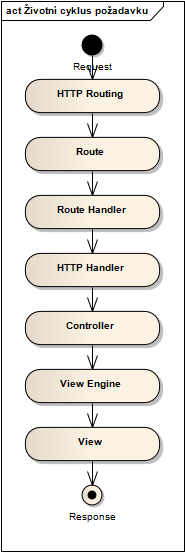
\includegraphics[scale=0.75]{figures/lifecycle}
\caption{Životní cyklus požadavku}
\label{fig:lifecycle}
\end{center}
\end{figure}

\subsection{Struktura modulu}
Každý modul musí mít danou strukturu, aby mohl být načten jádrem a správně fungovat.
Na obrázku \ref{fig:modulstruktura} je struktura vzorového modulu. Projekt je založený na standardní šabloně \textsf{ASP.NET MVC 3 Web Application}. Je třeba ji ale upravit, aby se nespouštěla samostatně, ale kompilovala se do adresáře \texttt{extension/plugins} v hlavním projektu \textsf{Core}. Toto se nastavuje v \texttt{Properties - Build - Output Path}. V \texttt{Properties} je třeba nastavit také záložku \texttt{Web}. Volba \texttt{Use Custom Web Server} se musí nastavit na vymyšlenou hodnotu. Konečně se musí změnit nastavení v Properties pod Solution Explorer (kliknutím na položku projektu) v položce \texttt{Always Start When Debugging} na \texttt{False}.

Také se musí do \texttt{References} přidat odkaz na projekt \textsf{Framework}, aby se daly využívat jeho třídy a rozhraní. Všem referencím je ale nutné zakázat kopírování na výstup ve vlastnostech. Všechny reference musí být uloženy na jednom místě v adresáři \texttt{bin} hlavního projektu \textsf{Core}. Dále se musí změnit vlastnosti všech souborů, které se nekompilují (zpravidla \texttt{Web.config}, \texttt{*.cshtml}, javacript, CSS a média). Ve vlastnostech u položky \texttt{Copy to Output Directory} je třeba nastavit \texttt{Copy Always}, protože by se jinak samy k aplikaci nepřidaly.

Další nastavení projektu budou ještě postupně přidávány, ale ve stručnosti jsou upraveny všechny soubory \texttt{Web.config}, \texttt{\_ViewStart.cshtml} a nový je soubor \texttt{Routes.cs}. Změny v souborech oproti standardnímu nastavení budou dále popsány. Soubory \texttt{Web.config} jsou v modulech jen pro přepsání rodiče pohledů a na import základních \textit{assemblies} a \textit{namespaces}.
\begin{figure}[h!]
\begin{center}
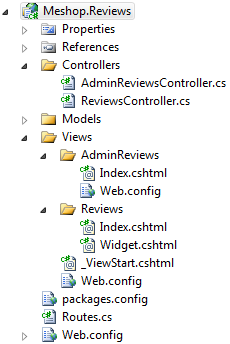
\includegraphics[scale=1]{figures/modulstruktura}
\caption{Struktura projektu modulu}
\label{fig:modulstruktura}
\end{center}
\end{figure}

\subsection{Připojení modulů}
\label{subsec:pripojenimodulu}

Připojování modulů je v aplikaci poloautomatické. Ve vývojovém režimu jde zcela automatizovat již výše zmíněným upravením nastavení při kompilování a spouštěním přímo v adresáři celého balíku projektů -- \textit{Solution}. To probíhá automaticky při spouštění při vývoji přímo z Visual Studia na vývojovém serveru IIS Express.

Po dlouhém hledání se mi podařilo najít článek Shannona Deminicka \cite{Shazwazza}, který se zabývá připojováním sestavení do jiných sestavení až po zkompilování. Proto jsem použil postup v něm navržený. Jde o systematické prohledávání daných adresářů a načítání tříd z nalezených sestavení, ještě než se spustí samotná aplikace. K tomu slouží soubor \texttt{PreApplicationInit.cs} popsaný výše v sekci \ref{sec:startapp}. vnitřní metoda celé moduly kopíruje do spouštěcího dočasného adresáře, protože se v původním adresáři zamknou a nejdou otevřít. Zároveň je třeba nastavit v balíčku \textsf{Core} v souboru \texttt{Web.config} v tagu \texttt{probing} atribut \texttt{privatePath} na adresář s dočasně nahranými moduly, aby mělo prostředí .NET informaci o dalším adresáři s dynamickými knihovnami.

Při kopírování sestavení do dočasného adresáře je vhodné ho při každé další kompilaci promazat. To se provede automaticky nastavením v Properties projektu modulu v záložce Build Events. Příkaz \texttt{rd /s /q "$(TargetDir)/../../temp/$(ProjectName)"} provede jeho smazání. Cesta je samozřejmě závislá na umístění projektu a adresáře pro moduly.

Jenže tím není vyhráno, protože se automaticky nenačtou do aplikace modulární služby, controllery a další implementace. K tomu se využívá IoC Kontejner \textsf{Castle.Windsor}, který třídy inicializuje, když je hledá ve hlavní aplikaci \textit{framework MVC}. Pomocí vlastní továrny je pak frameworku poskytne. Implementace používající kontejner je v souboru \texttt{Modules.cs}. Zdrojem pro načítání controllerů pomocí IoC Kontejneru byl článek od Mika Kolari \cite{kolari}. Staví na něm všechna rozšíření vlastního frameworku načítaná pomocí \textit{Dependency Injection}.

Statická třída \texttt{Modules} v souboru \texttt{Modules.cs} z balíčku \textsf{Framework} obsahuje metody, které jsou volány hlavně ve spouštěcí metodě \texttt{Application\_Start}. Všechny metody využívají společný Windsor IoC Kontejner, systematicky prohledávají všechna sestavení modulů a ukládají si implementace rozhraní a specifikace tříd, které jsou poté do aplikace \textit{injektovány}.
Metody zároveň hledají Routy pro aplikaci a adaptéry pro validační atributy.

\subsection{Body rozšíření}

V následujících podsekcích jsou probrány podrobně, ale s ohledem na omezení rozsahu, všechny body využité pro rozšíření aplikace pomocí modulů. Některé body mají implicitní implementace již v jádru, aby byla zajištěna správná funkčnost i bez modulů. Během vývoje jsem dospěl k myšlence, že všechny části, které jsou v jádru implicitní, by měly být pro přehlednost také umístěny do oddělených modulů, ale to by vyžadovalo složité přepracování, na které nezbyl během vývoje čas.

\subsubsection{Routy}
Rozšíření routování v aplikaci funguje paralelně s pevně daným routováním jádra. Rozšíření spočívá v dědění rozhraní \texttt{IRoutes} třídou v modulu -- umístěnou v \texttt{Routes.cs}.
Třída obsahuje předepsanou metodu, ve které jsou údaje o routách stejné jako v jádru aplikace -- viz ukázka \ref{list:route}. Načítání rout probíhá ve třídě \texttt{Modules} prohledáváním modulů a exekucí předepsaných metod ve třídách.

\subsubsection{Pohledy}
\label{subsec:pohledy}
Pohledy poskytují místo pro rozšíření pomocí rodičovských tříd, které ale dědí i pohledy v jádru. Pohledy představují v modulech nový problém. Nemohou totiž být vyhledány jako standardní pohledy v původním adresáři \texttt{Views} v jádře. Jsou totiž umístěny spolu se sestaveními v adresáři modulu.
Řešením je přepsání metod \texttt{View} a \texttt{PartialView} v kontroleru, které cesty k pohledům vracejí. Z tohoto důvodu vznikl controller \texttt{PluginController} určený ke specifikaci modulárními controllery. Idea je opět převzata z článku Mika Kolari\cite{kolari}.

Moduly obsahují shodnou strukturu pohledů jako jádro a musí také obsahovat soubor \texttt{Web.config} s určením, kterou třídu specifikují a jaké \textit{namespaces} implicitně používají. Jde použít i soubor
\texttt{\_ViewStart.cshtml} v adresáři \texttt{Shared} pro všechny pohledy. Soubor může měnit například základní šablonu \textit{layoutu}.

Také jsem přemýšlel o variantě kompilovat pohledy přímo do sestavení, postup byl ale nutný naučit každého, kdo by vyvíjel nový modul. Šlo o proces popsaný na blogu Chrise van de Steega\footnote{\url{http://www.chrisvandesteeg.nl/2010/11/22/embedding-pre-compiled-razor-views-in-your-dll/}}. Pro opuštění tohoto způsobu nahrává i výhoda možnosti úpravy pohledů v nezkompilovaných \textit{cshtml} souborech přímo na serveru.

\subsubsection{Formuláře}

Formuláře jsou obsaženy v pohledech, ale jejich vykreslení s modelem a vázání na model při příjmu je komplikované, proto jsem se zaměřil i na správnou implementaci formulářů v modulech. Mika Kolari\cite{kolari} úspěšně zkouší ve svém článku použít v modulech formulář. Jeho implementace se nachází v modulu \textsf{PageRating} upraveného tak, aby fungoval i v aplikaci e-shopu.

Dále jsem se obával spojení formulářů a widgetů \ref{sec:widgets}. Při testování spolupráce se ale nevyskytl žádný problém. Pro formuláře ve widgetech není třeba žádný speciální postup.

Ještě bych chtěl zmínit už zabudovanou funkčnost do formulářů přímo ve frameworku MVC. Jde o \textsf{Display} a \textsf{Editor Templates}. Na svém blogu ji popisuje Brad Wilson\footnote{\url{http://bitly.com/mvc2templates}}. Bohužel je návod ještě pro verzi MVC 2 a neobsahuje Razor šablony. Myšlenka spočívá v tom, že každá entita může mít svojí vlastní zobrazovací a formulářovou šablonu. Není tedy nutné vypisovat každý prvek entity do pohledu zvlášť. Ukázka \ref{list:settings} je z pohledu správy nastavení (šablona \texttt{Setting.cshtml}). Kód je ořezaný o HTML tagy tabulky. V souboru \texttt{Index.cshtml} je pak šablona použita na řádku \textbf{14} pomocí příkazu \texttt{Html.EditorForModel}. Framework rozpozná, o jakou jde entitu podle deklarace modelu.

\begin{lstlisting}[float=h!,language=HTML, caption={šablony pro formuláře}, label=list:settings]
<!--Views/Settings/EditorTemplates/Setting.cshtml-->
@model Meshop.Framework.Model.Setting
	@Html.DisplayFor(item => item.Key)
	@Html.HiddenFor(item => item.Key)
	@Html.EditorFor(item => item.Value)
	@Html.ValidationMessageFor(item => item.Value)

<!--Views/Settings/Index.cshtml-->
@model IList<Meshop.Framework.Model.Setting>
@using (Html.BeginForm()) {
    @Html.ValidationSummary(true)
    <fieldset>
        <legend>Settings</legend>
        @Html.EditorForModel()
        <input type="submit" value="Save" /> 
        @CommonService.Message
    </fieldset>
}
\end{lstlisting}

\subsubsection{Controllery}

Controllery jsou v modulech samozřejmostí. Jsou rozšiřitelné pomocí třídy \texttt{PluginController} zmíněné v části pohledů \ref{subsec:pohledy}. Bez dědění této třídy nebudou správně v modulech fungovat kvůli zmíněným pohledům.

Controllery jsou do aplikace načítány opět přes třídu \texttt{Modules} a využívá se \textit{Dependency Injection}. Načítají se pouze controllery dědící od \texttt{PluginController}. Může nastat situace, že některý modul bude obsahovat controller se stejným názvem. Konfliktu se lze vyhnout použitím namespaces v odkazech (generovaných příkazem \texttt{Html.ActionLink}) i v routách.

Stručná ukázka třídy \texttt{PluginController} \ref{list:plugincontroller} zobrazuje integraci připojení databáze a metod pro lokaci pohledů v modulech. Databázové spojení by mohlo být předěláno na šablonu Repository pro Unit testy. Týká se to všech jeho užití. V tom případě by se Repository \textit{injektovalo} ve třídě \texttt{Modules}. Co se týče hledání pohledů v modulech, využívá se reflexe a routovacího slovníku pro nalezení názvů adresářů a souboru. Výjimkové stavy jsou z ukázky pro přehlednost vypuštěny.

\begin{lstlisting}[float=h!,language=CSharp, caption={třída PluginController}, label=list:plugincontroller]
public abstract class PluginController : Controller
{
	protected DatabaseConnection2 db = new DatabaseConnection2();

    public new ViewResult View()
    {
        return base.View(ConstructViewPath());
    }
    private string ConstructViewPath(string viewName = "")
    {
        string viewPath = Modules.Path + GetAssemblyName() +"/";
        string ctrler = (string)RouteData.Values["Controller"];
        if (viewName == "") viewName = (string)RouteData.Values["Action"];
        return viewPath += "Views/" + ctrler  + "/" + viewName + ".cshtml";
    }   
}
\end{lstlisting}

\subsubsection{Služby}
\label{sec:services}
Služby jsou určeny pro distribuci dat controllerům a pohledům. Definice jejich rozhraní jsou v sestavení Framework. Služby jsou rozděleny podle zaměření:

\begin{itemize}
\item \texttt{IProduct} -- služby týkající se produktu. Jde o vyhledávání produktu v seznamu a další funkce. Služby v tomto případě představují příklad modelu.
\item \texttt{ICart} -- služba obsahuje všechny příkazy pro manipulaci s nákupním košíkem.
\item \texttt{ICategory} -- služba pro práci s kategoriemi.
\item \texttt{ICommon} -- služba poskytující funkce pohledům jak pro backend tak pro frontend. Jde o hodnoty z nastavení aplikace a informační zprávy. Zobrazení zprávy je vidět v ukázce \ref{list:settings} na řádku \textbf{16}. Služba je injektována do pohledů až za běhu aplikace při kompilaci pohledu s rodičem \texttt{BaseWebViewPage}.
\item \texttt{IFront} -- služby pro stránky ve frontendu. Jedná se hlavně o výpis položek hlavního Menu.
\item \texttt{IAdmin} -- služby pro stránky ve backendu. I zde se vypisují položky hlavního Menu.
\item \texttt{ICheckout} -- služba umožňující výměnu procesu \textit{checkoutu} za jiný. V její implementaci lze změnit odkazy na controller zajišťující \textit{checkout}.
\item \texttt{IListing} -- služby pro seznamy zboží vypsaných z kategorií. Tato služba nemá v základní aplikaci využití, protože zobrazování zboží nebylo nijak rozšiřováno.
\end{itemize}
 
Předpisy rozhraní by bylo samozřejmě nutné rozšířit v případě nasazení aplikace v ostrém prostředí. Služby jsou opět do controllerů \textit{injektovány} v třídě \texttt{Modules}. Pokud není implementace nalezena v modulech, použije se implicitní implementace v sestavení \textsf{Core}. Díky funkcím, kterými služby disponují, je možné nahradit modely službami.
 
\subsubsection{Menu}
\label{sec:menu}

V aplikaci jsou dvě rozšiřitelná menu. Položky menu jsou odkazy na metody controllerů, které jsou označeny atributem \texttt{Menu}. Jejich hledání probíhá v seznamu \textit{controllerů} poskytnutým třídou \texttt{Modules}. Pro frontend a backend se načítají menu zvlášť. Implementace jsou ve službách \texttt{DefaultFront} a \texttt{DefaultAdmin} implementujících rozhraní \texttt{IFront} a \texttt{IAdmin}. Atribut má možnost pojmenování. Samozřejmostí je překlad názvu podle lokalizace aplikace. Ukázka užití atributu \ref{list:menu} popisuje metodu v \texttt{HomeController}. 

\begin{lstlisting}[float=h!,language=CSharp, caption={atribut \texttt{Menu}}, label=list:menu]
[Menu(Name = "About")]
public ActionResult About()
{
    return View();
}
\end{lstlisting}


\subsubsection{Widgety}
\label{sec:widgets}

Widgety jsou grafické prvky v layoutu webové stránky. Dají se odebírat, přidávat a přemísťovat na různá místa různých stránek. Tabulka \ref{tab:pozice} ukazuje možnosti umístění ve stránce i ve specifických pohledech. 

Widgety fungují stejně jako běžné metody v controllerech, ale jsou opatřeny tagy \texttt{Child\-Action\-Only} a \texttt{Placement}. Potřebují mít tedy i vlastní pohled. Widgety zároveň mohou být v jádru i v modulech.

\begin{itemize}
\item \texttt{ChildActionOnly} -- vestavěný atribut, který dovoluje spustit metodu jako vnořenou, nejde volat přímo pomocí URL.
\item \texttt{Placement} -- určuje na jakém místě se obsah metody objeví. Tabulka \ref{tab:pozice} ukazuje možnosti umístění pomocí parametrů \textit{Position} a \textit{Template} (pohled). Možnosti jsou zapsány v typech enum -- \texttt{PagePosition} a \texttt{PageTemplate}.
\end{itemize}

\begin{table}
\centering
\begin{tabular}[c]{|c|c|}
\hline 
\textbf{Position} & \textbf{Template} \\ 
\hline 
Left & Index \\ 
\hline 
Right & Product \\ 
\hline 
Bottom & Catalog \\ 
\hline 
Top & Cart \\ 
\hline 
Header & Login \\ 
\hline 
Footer & Address \\ 
\hline 
Document & Shipping \\ 
\hline 
• & Payment \\ 
\hline 
• & Search \\ 
\hline 
• & All \\ 
\hline 
\end{tabular}
\caption{Možnosti umístění Widgetů}
\label{tab:pozice}
\end{table} 

Widgety se načítají z controllerů podobně jako položky menu. Třída \texttt{DefaultWidgetter} se načte při načítání stránky, prohledá seznam controllerů a zjistí atributy jejich metod. Poté se na určitých místech ve stránce volají pomocí metody \texttt{WidgetPlace}. Ta je ovšem pouze delegátem a implementací je metoda \texttt{Compose} ve třídě \texttt{DefaultWidgetter}.

V metodě \texttt{Compose} se poté volá vestavěná metoda \texttt{RenderAction}, která zajistí zobrazení widgetu. Aplikace takto ale prochází znova životním cyklem. Ten se provede tolikrát, kolik je na stránce widgetů. Může se tak jednat o zásadní zpomalení aplikace. Toto je ale jediný dostupný způsob, který poskytuje všechny možnosti akce controlleru i s modelem a formuláři.

Zlepšením implementace by určitě bylo kešování seznamu widgetů a jiný způsob načítání. Pro ilustraci komplexnosti mechanismu je uveden sekvenční diagram \ref{fig:widgety}. Stereotyp \textit{<<recursion>>} představuje nové volání metody v controlleru, tedy nový životní cyklus.

\begin{figure}[h!]
\begin{center}
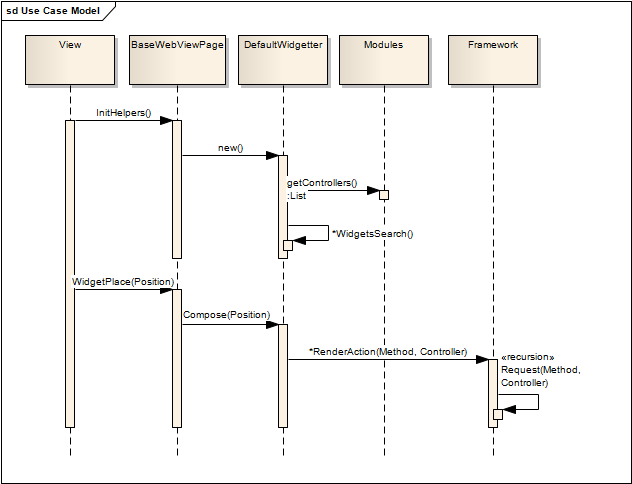
\includegraphics[scale=0.71]{figures/widgety}
\caption{Sekvenční diagram zobrazování widgetů}
\label{fig:widgety}
\end{center}
\end{figure}

\subsubsection{Entity}
\label{subsec:pripojenientit}
I entity se dají rozšířit. V základu aplikace nebylo této schopnosti využito, ale pro praktickou implementaci je toto třeba. Způsob rozšíření entit je rozdělen interně na 3 způsoby, ale vždy využívá mechanismu dědění původní entity. Detaily nastavení jsou probírány v článcích na blogu Morteza Manavi\footnote{\url{http://bit.ly/CodeFirstInheritance}}.

Připojení demonstruje entita \texttt{Review} z modulu \textsf{Reviews}. Implementovat injekci entit bylo možné jen díky článku publikovaném jako návodu na psaní modulů pro projekt NopCommerce \cite{NOPE}. Nikde jinde, ani v dokumentačních materiálech Entity Frameworku tato možnost zmíněna není, což považuji za velkou slabost dokumentace Entity Frameworku.

Způsob implementace postupuje podle příkladu z článku \cite{NOPE}. Nejprve je třeba vytvořit třídu s entitou specifikující třídu \texttt{PluginEntity}, poté konfiguraci entity podle příkladu specifikující \texttt{Entity\-Type\-Configuration}. Oboje se budou injektovat do \texttt{DbContext} v metodě \texttt{OnModel\-Creating}. Dále je možné do aplikace nahrát prvotní obsah entity přes implementaci rozhraní \texttt{IDbSeed}, které se injektuje do souboru inicializace databáze. Databáze se bohužel stane nekompatibilní, protože se změní model, viz. popis Entity Frameworku \ref{sec:ef}.

Dotazování na tyto modulární entity z \texttt{DbContext} pak probíhá jinak, rozdíl demonstruje ukázka \ref{list:rozdilentit}. Rozšiřující entita je získávána z \texttt{DbContext} na řádku \textbf{5} a z ní pak základní entita na řádku \textbf{6}. 

Nevýhodou je nemožnost pracovat s rozšiřujícími entitami v jiných modulech, o jádře ani nemluvě.

\begin{lstlisting}[float=h!,language=CSharp, caption={rozdíl použití základní a rozšiřující entity}, label=list:rozdilentit]
[ChildActionOnly]
[Placement(Position = PagePosition.Document, Template = PageTemplate.Index)]
public ActionResult Widget()
{
    var review = db.Set<Review>().First();
    ViewBag.CustomerMail = review.Customer.Email;
    return PartialView(review);
}
\end{lstlisting}

\subsubsection{Frontend}

Frontend je rozšiřitelný pomocí výše zmiňovaných bodů. Základem rozšiřování je upravování pohledů frontendu, které nejsou zkompilované. Další možnost je dopisování controllerů a jejich pohledů. Odkazy na akce se přidají následně do menu frontendu

\subsubsection{Backend -- administrace}
\label{subsub:backend}
Backend, nebo-li administrace, je rozšiřitelná stejně jako frontend s tím rozdílem, že musí být zabezpečená atributem \texttt{Admin}. Nemůže totiž dědit současně od \texttt{PluginController} a \texttt{AdminController}. \texttt{PluginController} má proto přednost. Nabízí se možnost vytvoření \texttt{AdminPluginController}, který by dědil od jedné třídy a obsahoval manuálně dopsané \textit{metody} a \textit{properties} druhé třídy. 

Controller se poté opět musí přidat do menu backendu stejným atributem \texttt{Menu}, rozdíl spočívá v detekci atributu \texttt{Admin}. 

\subsection{Omezení modulů}

Omezení byla postupně zmiňována v podsekcích Modulů \ref{sec:moduly}. Zde jsou shrnuty.

\begin{itemize}
\item \textbf{Entity} -- rozšíření entit je možné pouze v rámci modulu. Mimo něj Entita viditelná není. Viz. \ref{subsec:pripojenientit}. Pokud by se entita deklarovala jinde, dojde ke konfliktům a duplikaci.
\item \textbf{Widgety} -- omezené umístěním na určená místa a omezují výkonnost aplikace, viz. \ref{sec:widgets}.
\item \textbf{AdminPluginController} -- zmíněný výše v \ref{subsub:backend}. Přesněji jde o vícenásobnou dědičnost, která není v .NET možná. Je třeba sáhnout k rozhraní a duplicitní implementaci.
\item \textbf{Služby} -- rozšíření služeb musí být provedeno ve frameworku aplikace, který je třeba znova zkompilovat. Modulárním způsobem je možné pouze implementovat rozhraní.
\item \textbf{Kopie do modulu} -- všem souborům, které se v modulech nekompilují je třeba nastavit manuálně kopírování do adresáře se zkompilovaným modulem.
\end{itemize}



\section{Spuštění aplikace}
\label{sec:spusteni}
Spuštění aplikace rozlišuje nejméně dva způsoby. Jedním je debug mód, který se spouští přímo ve Visual Studiu a druhým je mód release, který je určený pro ostrý provoz na serveru.

Pro spuštění ve Visual Studiu je třeba následovat některý z instalačních tutoriálú pro ASP.NET MVC 3. Nejlepší je přímo na oficiální stránce\footnote{\url{http://asp.net/mvc/mvc3}}. Nejlepší volbou je stažení \textit{Web Platform Installer} (WPI) z odkazu v návodu. Ten nabídne instalaci všech základních částí včetně Visual Studia ve verzi zdarma. Poté při otevření \textsf{solution} (balík projektů celé aplikace pro Visual Studio) se vyřeší závislosti na jiných knihovnách potřebných k běhu aplikace.

Pro urychlení instalací doplňků je vhodné zaškrtnout při instalaci WPI i instalaci serveru IIS Express a databázového enginu SQL Server Compact.

Pro spuštění na serveru IIS nebo na hostingu je třeba, aby byl server vybaven stejnými technologiemi, tedy ASP.NET 4, MVC 3 a SQL Server Compact. V případě nepřítomnosti frameworku MVC 3 je možné jej nahrát přímo s aplikací. Postup pro nahrání aplikace na IIS je dostupný také v tutoriálech na oficiálních stránkách\footnote{\url{http://www.asp.net/mvc/overview/deployment}}.

Také je důležité, aby server poskytoval plná práva \textbf{Full Trust}\footnote{\url{http://msdn.microsoft.com/en-us/library/wyts434y.aspx}} z důvodu používání IoC kontejneru Castle Windsor, který je vyžaduje. Požadavky na plná práva bohužel vyřazují velké množství webhostingů. Dále je nutné povolit zápis do adresáře \texttt{App\_Data}, kde je uložen databázový soubor a také zápis do adresáře modulů \texttt{extensions/temp}.



\subsection{Instalace a odebrání modulu}
\label{sec:instalace}
Při instalaci nebo odebírání modulů je třeba vypráznit \textsf{Application Pool} (keš) v IIS příkazem \textsf{Recycle}. Toto se ale ukázalo jako nefunkční řešení v případě nepřekompilování projektu \textsf{Meshop.Core}. Proto se musí vymazat aplikace z adresáře \texttt{C:\symbol{92}Windows\symbol{92}Microsoft.NET\\\symbol{92}Framework\symbol{92}v4.0.30319\symbol{92}Temporary ASP.NET Files\symbol{92}} .

Instalace modulu se provádí zkompilováním modulu a spolu se soubory pohledů a dalšími se nakopíruje do aplikace do adresáře \texttt{extensions/plugins/Meshop.\{Modul\}}. Knihovna modulu v tomto případě musí mít název \texttt{Meshop.\{Modul\}.dll}. Zkompiluje se tak v případě názvu projektu modulu \textsf{Meshop.\{Modul\}}. Při spuštění se adresáře pluginů zkopírují do adresáře \texttt{extensions/temp} ze kterých se načtou.

Při odebírání modulu je nutné kromě vymazání keše a restartu aplikace také vymazání adresáře pluginu z obou adresářů \texttt{extensions/temp} i \texttt{extensions/plugins}.

Data v databázi se při změně v modulech vymažou a načtou se data z třídy \texttt{Database\-Initializer} a tříd implementujích rozhraní \texttt{IDbSeed}. Toto chování je bohužel nastaveno z důvodu absence funkce \textsf{Migrations} v Entity Frameworku 4.1, viz. \ref{sec:ef}.

%*****************************************************************************
\chapter{Testování}
\label{sec:testovani}

Při a po vývoji aplikace probíhalo několik různých testování. Během vývoje byly postupně testovány všechny implementované funkce a jejich vzájemná součinnost. Pomocí těchto implementačních testů byla odhalena různá omezení, byly opraveny četné chyby a ošetřeny výjimky.

Zajímavější ovšem bylo testování nasazení na ostrý webový server, testování výkonu a uživatelský test.

\section{Testování nasazení}

Nasazení na ostrý webový server by se podle předpokladů nemělo zásadně lišit od vývojového prostředí. Při testování byla použita finální verze aplikace včetně testovacích modulů \textsf{Reviews} a \textsf{PageRating}. Otestovány byly webhosting \emph{Aspone.cz}\footnote{\url{http://www.aspone.cz/}} a vlastní IIS server na osobním počítači.

\subsection{Free webhosting Aspone.cz}
Program \emph{Freehosting} na serveru \emph{Aspone.cz} je zdarma a poskytuje všechny potřebné služby pro aplikaci. Bylo provedeno zkušební nasazení a zkopírovány potřebné soubory (na DVD v adresáři \texttt{web}) na registrovanou službu s adresou \url{http://modular.aspone.cz}. Spuštění má proběhnout automaticky po nahrání souborů na privátní úložiště FTP.

Při načítání webu z prohlížeče se vyskytla inicializační chyba. Knihovna \textbf{Castle Windsor}, použitá jako IOC kontejner, způsobila nezdokumentovanou chybu \uv{\emph{{System.Type\-Load\-Exception:} Inheritance security rules violated while overriding member}}. Z dotazů týkajících se této chyby na webu stackoverflow.com\footnote{\url{http://stackoverflow.com/questions/3928727/windsor-2-5-does-not-work-in-medium-trust}} vyplývá, že Castle Windsor nezvládne běžet v poslední verzi .NET frameworku s bezpečnostními omezeními na úrovni \textit{Medium Trust}. K běhu je potřeba oprávnění \textit{Full Trust}. 

Při vybírání IOC kontejneru Castle Windsor nebylo toto omezení nikde v dokumentaci zmíněno. Z testování vyplynulo, že tento IOC kontejner není vhodný pro aplikaci běžící na jiné úrovni než \textit{Full Trust}. To by vyžadovalo pořízení placené varianty webhostingu Aspone.cz, které už \textit{Full Trust} podporují. Jiné hostingy\footnote{\url{http://www.web4u.cz}} bohužel nenabízejí \textit{Full Trust} ani v nejvyšších placených variantách.

\subsection{Vlastní IIS server}
Tato varianta testování byla zvolena po neúspěšném nasazení aplikace na webový hosting bez úrovně \textit{Full Trust}. Byl nainstalován IIS na systém Windows 7 Professional a byl doplněn o potřebné knihovny pomocí \textit{Instalační služby webové platformy} (WPI). Byly nainstalovány následující vyžadované knihovny:

\begin{itemize}
\item ASP.NET MVC 3
\item Microsoft SQL Server Compact 4.0
\item Jazykové sady ASP.NET MVC 3
\end{itemize}

Dále byl přidán nový \textit{Web}. Byla upravena oprávnění přístupu pro adresáře \texttt{App\_Data}, kvůli přístupu k databázi, a \texttt{extensions/temp}, aby mohl server vytvářet pracovní kopie modulů. Také byla nastavena \textit{Úroveň důvěryhodnosti rozhraní .NET} na \textbf{Full}. \textit{Fond aplikace} byl zvolen \textit{DefaultAppPool} s verzí rozhraní \textbf{v4.0(integrated)}. Aplikace byla nastavena tak, aby byla dostupná na adrese \textit{localhost}.

Při testování byla nejprve spuštěna aplikace s moduly a všechny funkčnosti byly dostupné. V druhém kroku byly pluginy z adresáře odebrány a aplikace byla restartována, všechny funkčnosti také běžely v pořádku.

\label{test:problem}
Ve třetím kroku byly opět moduly přidány a aplikace byla restartována, jenže nastala chyba, která naznačovala, že moduly do aplikace nahrány nebyly. Byly prozkoumány všechny způsoby kešování a recyklace keše. Pomohlo až překompilování projektu jádra a přehrání souboru \texttt{Meshop.Core.dll}. Později při uživatelských testech s vývojáři byla nalezena další varianta. Jde o vymazání keše manuálně. Obnoví se tak Fond Aplikací IIS serveru. Keš aplikací je umístěna v adresáři 
\\\texttt{C:\symbol{92}Windows\symbol{92}Microsoft.NET\symbol{92}Framework\symbol{92}v4.0.30319\symbol{92}Temporary ASP.NET Files\symbol{92}}. 
\\Cesta se liší u 64-bitové verze serveru v adresáři -- \texttt{Framework64}. Pro správný běh stačí před smazáním aplikaci zastavit a poté ji již s moduly spustit. 

Zajímavé je, že aplikace funguje po odebrání modulů i bez vymazání keše.\\



Z testování nasazení aplikace na produkční server vyplývá, že jsou na server kladeny vyšší nároky. Jde o vlastní nastavení serveru a možnost manuálně mazat keš ASP.NET frameworku. Běžné webhostingové programy pro tuto aplikaci nestačí. Je třeba sáhnout po pokročilejších programech nebo zvolit vlastní řešení serveru.

\section{Testování doby odpovědi}

Doba odpovědi znamená dobu, za kterou se načte vyžádaná webová stránka. Testování probíhalo na vývojovém serveru IIS Express a na serveru IIS. Byly načítány stránky s obsahem z modulů i bez. Aplikace byla v jednom případě s moduly, ve druhém bez modulů. Následující tabulky \ref{tab:testIISE} a \ref{tab:testIIS} zobrazují doby odpovědí prvního načtení a dalších načtení. Před každým testováním byla vymazána keš.

K měření byla využita funkce \textit{Timing} debugovacího modulu \textsf{Glimpse} přímo na stránce aplikace, viz. sekce \ref{glimpse}.


\begin{table}[h!]
\centering
\begin{tabular}[c]{|c||c|c||c|c|}
\hline
 & \multicolumn{2}{c||}{\textbf{s moduly}} & \multicolumn{2}{|c|}{\textbf{bez modulů}} \\
\hline 
\multirow{2}{*}{\textbf{stránka}} & \textbf{1. načtení} & \textbf{2. načtení} & \textbf{1. načtení} & \textbf{2. načtení} \\ 
& [ms] & [ms] & [ms] & [ms] \\
\hline 
Home         & 4,62s  & 323 & 3,23s & 241 \\ 
\hline 
About        & 217  & 185 & 178 & 133 \\ 
\hline 
Reviews      & 547  & 179 & -- & -- \\ 
\hline 
1. kategorie & 343  & 263 & 305 & 204 \\ 
\hline 
\end{tabular}
\caption{Doba odpovědi v IIS Express}
\label{tab:testIISE}
\end{table} 


\begin{table}[h!]
\centering
\begin{tabular}[c]{|c||c|c||c|c|}
\hline
 & \multicolumn{2}{c||}{\textbf{s moduly}} & \multicolumn{2}{|c|}{\textbf{bez modulů}} \\
\hline 
\multirow{2}{*}{\textbf{stránka}} & \textbf{1. načtení} & \textbf{2. načtení} & \textbf{1. načtení} & \textbf{2. načtení} \\ 
& [ms] & [ms] & [ms] & [ms] \\
\hline 
Home         & 4,66s  & 165 & 4,2s & 203 \\ 
\hline 
About        & 230  & 115 & 140 & 114 \\ 
\hline 
Reviews      & 506  & 146 & -- & -- \\ 
\hline 
1. kategorie & 459  & 205 & 552 & 169 \\ 
\hline 
\end{tabular}
\caption{Doba odpovědi v IIS}
\label{tab:testIIS}
\end{table} 

Při měření dosahovaly další načtení stránek velmi podobných hodnot jako při druhém načtení. Rozdíl byl pouze v milisekundách. To je způsobeno dynamickou kompilací pohledu při prvním načítání a použití zkompilovaného pohledu při dalších načítáních. Tomuto zpoždění lze předejít zkompilováním pohledů přímo do \textit{assembly}, viz. sekce \ref{subsec:pohledy}.

Další nepatrné zpoždění je pozorovatelné při načítání stránek v IIS Express v aplikaci s moduly a bez modulů. Na IIS serveru se ovšem toto zpoždění již neprojevuje. Pravděpodobně je to díky tomu, že je IIS optimalizovaný pro ostré nasazení. Může jít ovšem také o vytížení procesoru a vznikne tak rozdíl pár desítek ms. 

V průměru se doba odpovědi pohybuje kolem 200ms u zkompilovaných pohledů, což je rychlá reakce z pohledu uživatele. Stránka \texttt{Home} obsahuje 3 widgety -- jeden z modulu \textsf{Reviews} -- a její doba odpovědi se zásadně neliší. Samozřejmě nelze vyloučit, že se doba odpovědi zvedne při implementaci dalších funkcí do aplikace. Dobu může zvednout i přidávání modulů a narůstání dotazů do databáze. Aplikaci je ale možné dále optimalizovat. 

Závěrem testování doby odpovědi lze říci, že testovací moduly neprokázaly na serveru IIS zvýšenou reakční dobu díky kešování. Také byla vyvrácena hypotéza, že widgety zásadně prodlužují reakční dobu, viz. \ref{sec:widgets}.



\section{Uživatelský test}
Tento uživatelský test se týkal otestování tvorby modulu zkušenými vývojáři v prostředí platformy .NET a jeho nasazení na vývojové verzi aplikace. Testovaní vývojáři také zkoušeli moduly odebírat a přidávat.

Vývojáři byli dva spolužáci, kteří používají platformu .NET na pokročilé úrovni a mají přehled o platformě i o Visual Studiu. Oba vývojáři dostali instrukce jak moduly instalovat a odebírat. Druhý vývojář také vytvořil základní strukturu modulu a úspěšně jej instaloval do aplikace. Testování probíhalo ve Visual Studiu 2010 a aplikace se spouštěla na vývojovém serveru IIS Express.

První zkoušený vývojář prošel testem tak, že nainstaloval závislosti do Visual Studia a načetl projekty. Poté provedl spuštění aplikace i s moduly. V dalším kroku moduly odstranil a aplikaci opět spustil. Ve třetím kroku moduly do aplikace přidal a vznikl již dříve popisovaný problém \ref{test:problem}, který se vyřešil překompilováním knihovny jádra. Později bylo nalezeno umístění keše ASP.NET frameworku.

Druhý vývojář testoval nasazení aplikace v připraveném Visual Studiu s nainstalovanými závislostmi a prošel všemi kroky stejně. Navíc ještě naprogramoval podle instrukcí vlastní modul, který pak přidal k aplikaci.

Podle reakcí testovaných vývojářů lze říci, že je možné modulární aplikaci publikovat pro další vývojáře, kteří jí budou moci dále rozšířit.


\section{Srovnání s existujícími řešeními}

Nejbližší existující řešení je \textit{nopCommerce}, protože je také vyvíjeno pro platformu Microsoft .NET, viz. sekce \ref{nop}. 

Aplikace \textit{nopCommerce} má velikou základnu uživatelů a proto jsou její chyby a nedostatky rychleji odhaleny. Je pro ni vyvinuto velké množství modulů a pracuje na ní tým 15-ti lidí už více jak 3 roky, z toho její zakladatel na plný úvazek.

Aplikace \textit{nopCommerce} ale nebyla nainstalována lokálně. Byly vyzkoušeny pouze verze online uvedené v referencích. Nejrychlejší reakce měl první web \\ \url{http://www.yourpersonaljeweller.co.uk/}, který načetl stránku bez grafiky v rozmezí 165ms až 1s. Z toho lze usoudit, že je obchod i přes množství funkčností dobře optimalizovaný. Server IIS 6.0, na kterém aplikace běží, musí být také dobře optimalizovaný. Doba také navíc zahrnuje zpoždění přenosu dat ze vzdáleného serveru.

Lze konstatovat, že při konstantním vývoji aplikace modulárního e-shopu více vývojáři, by se mohla stát v budoucnu konkurenceschopnou aplikaci \textit{nopCommerce}. Zatím se jedná pouze o testovací prototyp.


%*****************************************************************************
\chapter{Závěr}
\label{sec:zaver}

\section{Zhodnocení}

V této práci byla navrhnuta a úspěšně implementována aplikace e-shopu s využitím modulární architektury. Práce se soustředila na možnosti rozšiřitelnosti aplikace a ověřila, že je tvorba takového internetového obchodu možná. Všechny základní požadavky kladené na aplikaci z hlediska rozšiřitelnosti se podařilo splnit. Zvolená vývojová platforma Microsoft .NET poskytla nejen dostatek funkcí, ale i integrované nástroje v podobě kvalitního vývojového prostředí, jakým je \textit{Visual Studio}.

Rešerše poskytla náhled do prostředí elektronického obchodování a bylo zjištěno, že nabídka elektronických obchodů je doslova obrovská. Byla nalezena velmi kvalitní ale i nekvalitní řešení. V testech bylo ověřeno, že i volně dostupné řešení elektronického obchodu může být kvalitní.

Pro implementaci byla zvolena architektura MVC, kterou poskytuje platforma Microsoft .NET jako rozšiřující framework ASP.NET MVC ve verzi 3. Framework nabídl mnoho možností pro rozšíření a umožnil tvorbu modulární aplikace ve spolupráci s návrhovým vzorem \textit{Dependency injection} a funkcemi platformy Microsoft .NET. Platforma se ukázala jako dobře zvolená, protože je velmi rozšířená a její vývoj neustále pokračuje. Platforma je dobře zdokumentovaná a pro mnoho problémů je dostupné řešení na oficiálních i komunitních webových stránkách. Učící křivka ale vzhledem k rozsáhlosti platformy z počátku stoupá velmi pozvolna. S pokročilými funkcemi frameworku ASP.NET MVC 3 pomohla i zakoupená kniha \cite{MVC1}.

Rozšíření jádra aplikace pomocí modulů bylo dosaženo přes body rozšíření. Lze tak mimo jiné rozšířit datový model aplikace, přidávat další webové stránky, doplňovat existující stránky, nebo je kompletně nahrazovat. 

Testování prokázalo, že moduly nemají na aplikaci při načítání webových stránek vliv. Během testů byla objevena omezení, která vyžadují nasazení aplikace na webový server s vlastní správou nebo využití pokročilých webhostingových programů. Omezení se týkají externí knihovny Castle Windsor pro načítání modulů a webového serveru IIS. 

Uživatelský test s vývojáři potvrdil, že je aplikaci možné poskytnout dalším vývojářům, kteří ji dál mohou rozšířit o další moduly a funkce. Dalším vývojem by tak mohl vzniknout z funkčního prototypu plnohodnotný modulární elektronický obchod.



%Zhodnocení splnění cílů práce a vlastního přínosu práce 
%(při formulaci je třeba vzít v potaz zadání práce)

\section{Rozšíření}

Aplikace modulárního e-shopu byla implementována jako funkční prototyp. Poskytuje tak dostatek místa pro její další rozšíření. 

Pokračování práce by se mohlo věnovat optimalizaci výkonu aplikace, zejména části načítání modulů a optimalizovat její funkce. Dále by bylo vhodné vyřešit omezení objevená při testování prototypu. To by si vyžádalo rešerši mezi dostupnými IoC kontejnery, jakým je i použitý Castle Windsor, a volbu toho nejvhodnějšího z hlediska výkonu, funkcí a omezení. Aplikace by také mohla být optimalizována implementací kešování zdrojů načítaných do webových stránek.

Dalším vhodným rozšířením by mohl být systém pro katalogizaci dostupných modulů, jakým je například balíčkový systém \textit{NuGet} pro Visual Studio. %, zmíněný v sekci \ref{subsec:roz}.
Systém by mohl dále umožnit rozšíření existujících modulů dalšími moduly.

Z důvodu větší přehlednosti by bylo také praktické přesunout základní rozhraní z jádra do modulů. Pro úspěšné nasazení aplikace je ale nejdůležitější rozšíření o moduly, které z prototypu udělají v praxi použitelný elektronický obchod.



%*****************************************************************************
% Seznam literatury je v samostatnem souboru reference.bib. Ten
% upravte dle vlastnich potreb, potom zpracujte (a do textu
% zapracujte) pomoci prikazu bibtex a nasledne pdflatex (nebo
% latex). Druhy z nich alespon 2x, aby se poresily odkazy.

% originally following specification for bibliography formating was used
%\bibliographystyle{abbrv}

% Here is an improvment by Petr Dlouhy (April 2010).
% It is mainly for supervisors who expect Czech fomrating rules for references
% Additional feature is live url addresses to sources from your pdf file
% It requires the file csplainnat.bst (included in this sample zipfile).

\bibliographystyle{csplainnat}

%bibliographystyle{plain}
%\bibliographystyle{psc}
{
%JZ: 11.12.2008 Kdo chce mit v techto ukazkovych odkazech take odkaz na CSTeX:
\def\CS{$\cal C\kern-0.1667em\lower.5ex\hbox{$\cal S$}\kern-0.075em $}
\bibliography{reference}
}


%*****************************************************************************
%*****************************************************************************
\appendix

%*****************************************************************************
\chapter{Seznam použitých zkratek}

\begin{description}
\item[ADO.NET] ActiveX Data Objects .NET
\item[AJAX] Asynchronous JavaScript and XML
\item[APEK] Asociace pro Elektronickou Komerci
\item[API] Application Programming Interface
\item[ASP.NET] Active Server Pages .NET
\item[CGI] Common Gate Interface
\item[CMS] Content Management System
\item[CSS] Cascading Style Sheets
\item[DDL] Data Definition Language
\item[DI] Dependency Injection
\item[DVD] Digital Versatile (Video) Disc
\item[ECMA] European Computer Manufacturers Association 
\item[EDM] Entity Data Model
\item[EE] Enterprise Edition
\item[EF] Entity Framework
\item[ER] Entity-Relationship
\item[FTP] File Transfer Protocol
\item[HTML] HyperText Markup Language
\item[HTTP] HyperText Transfer Protocol
\item[IEEE] Institute of Electrical and Electronics Engineers 
\item[IDE] Integrated Development Environment
\item[IIS] Internet Information Services
\item[IOC] Inversion of Control
\item[IT] Information Technology
\item[LINQ] Language Integrated Query
\item[MSDN] Microsoft Developer Network
\item[MVC] Model-View-Controller
\item[NAS] Network Attached Storage
\item[ORM] Object-Relational Mapping
\item[PHP] Hypertext Preprocessor
\item[SAP] Systeme, Anwendungen, Produkte in der Datenverarbeitung
\item[SEO] Search Engine Optimization
\item[SMS] Short Message Service
\item[SOC] Separation of Concerns
\item[SQL] Structured Query Language
\item[SSL] Secure Sockets Layer
\item[URI] Uniform Resource Identifier
\item[URL] Uniform Resource Locator
\item[UX] User eXperience
\item[WPI] Web Platform Installer
\item[XML] eXtensible Markup Language


\end{description}


%*****************************************************************************
\chapter{Ukázky aplikace}

\begin{figure}[h!]
\begin{center}
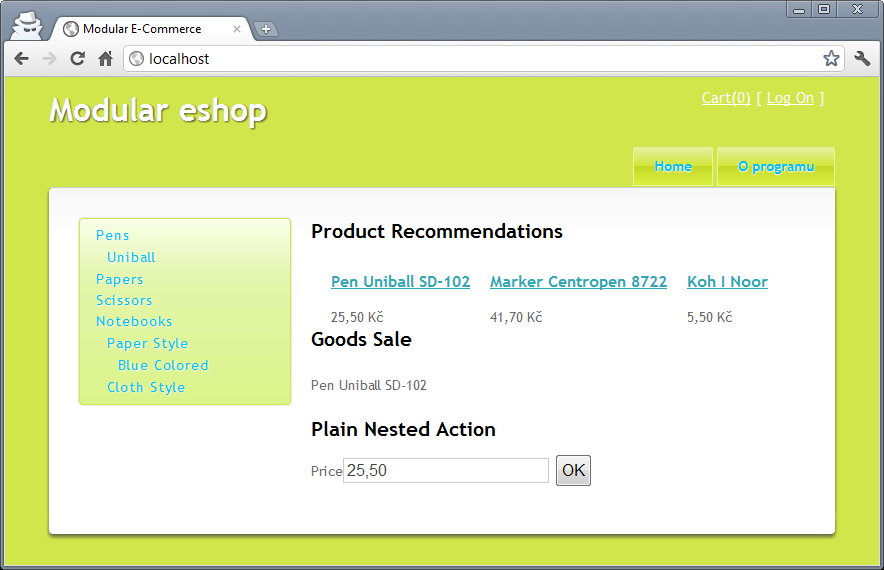
\includegraphics[scale=0.65,angle=0]{figures/frontend1}
\caption{Ukázka frontendu bez modulů}
\end{center}
\end{figure}

\begin{figure}[h!]
\begin{center}
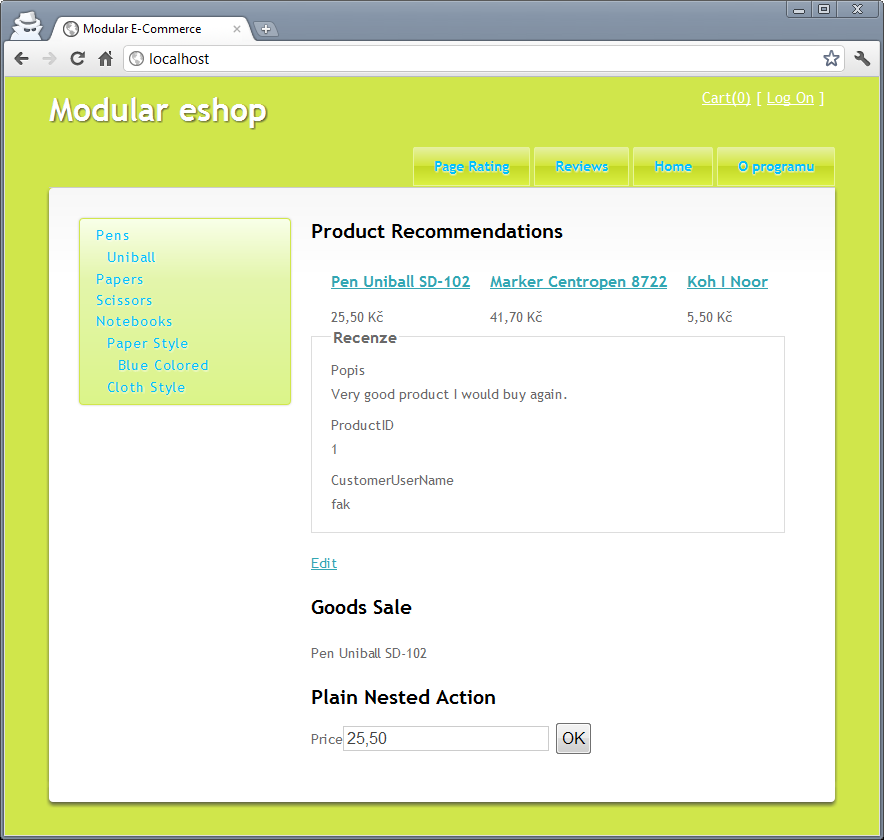
\includegraphics[scale=0.65,angle=0]{figures/frontend2}
\caption{Ukázka frontendu s moduly}
\end{center}
\end{figure}

\begin{figure}[h!]
\begin{center}
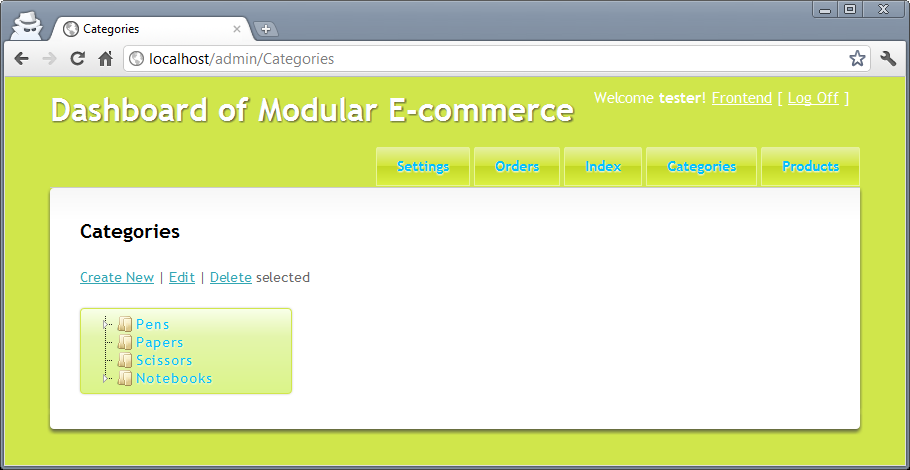
\includegraphics[scale=0.65,angle=0]{figures/backend1}
\caption{Ukázka backendu bez modulů}
\end{center}
\end{figure}

\begin{figure}[h!]
\begin{center}
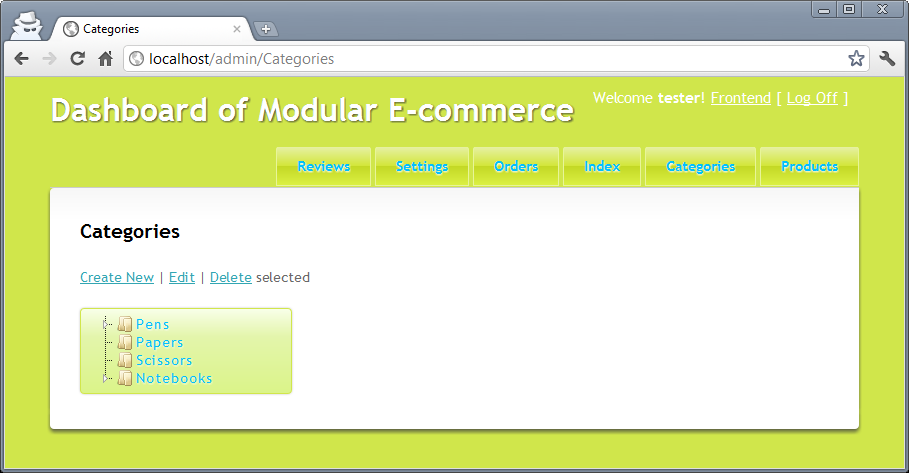
\includegraphics[scale=0.65,angle=0]{figures/backend2}
\caption{Ukázka backendu s moduly}
\end{center}
\end{figure}

%*****************************************************************************
\chapter{Instalační a uživatelská příručka}

Instrukce pro instalaci a spuštění aplikace jsou z textu práce pro přehlednost extrahovány do této přílohy.

\section{Instalace prostředí}
Operační systém musí být nejlépe Windows 7. Jsou možné i starší verze. Musí mít ale nainstalovaný Microsoft .NET 4.
Dále je nutné doinstalovat ASP.NET 4, Visual Studio 2010 nebo Visual Web Developer 2010.

\begin{enumerate}
\item Stáhněte instalační balík z webu \url{http://www.asp.net/mvc} -- Web Platform Installer (WPI), který následně spusťte a obrňte se trpělivostí.
% \begin{figure}
% \begin{center}
% 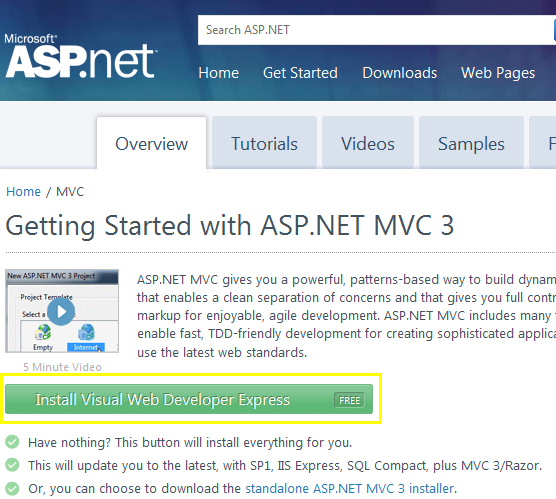
\includegraphics[scale=0.65,angle=0]{figures/aspnetmvc}
% \caption{Stažení balíku WPI}
% \end{center}
% \end{figure}

% \begin{figure}
% \begin{center}
% 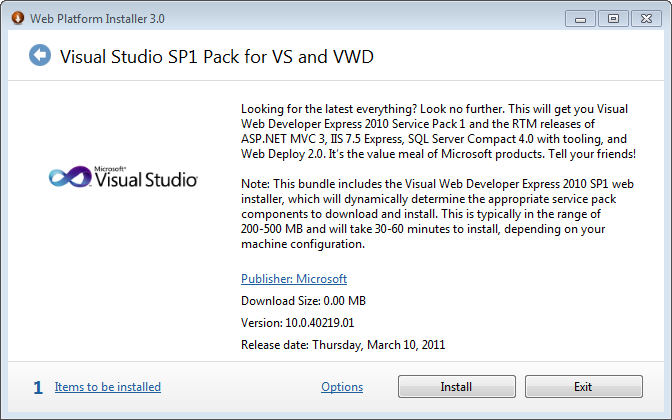
\includegraphics[scale=0.65,angle=0]{figures/wpi}
% \caption{Instalace balíku WPI}
% \end{center}
% \end{figure}

\item Spusťte Visual Studio 2010 Express, nebo pokud je vlastníte, tak některou z plných verzí.
\item Načtěte soubor \texttt{Meshop.sln} a v případě edice \textit{Express} potvrďte všechna hlášení -- i chybová.

\end{enumerate}




\section{Instalace aplikace}
Aplikace se instaluje pouhým přehráním do určeného adresáře webového serveru.
Pokud nejde o webový hosting, musí se nastavit v IIS manageru (správci) příslušné nastavení. IIS server je zabudovaný ve Windows 7 Professional nebo ve Windows Server 2008.
Pro~vyzkoušení aplikace ale plně postačí vývojové prostředí Visual Studio 2010.

Nastavení webového serveru:
\begin{enumerate}
\item Spusťte IIS Manager (\texttt{InetMgr.exe})
\item Přidejte aplikaci (\textit{Add Web Site}/\textit{Přidat web}) a zvolte cestu k aplikaci.
\item Nastavte \textit{.NET Trust Level}/\textit{Úrovně důvěryhodnosti rozhraní .NET} na \textbf{Full}.
\item Nastavte adresářům \texttt{App\_Data} a \texttt{extensions/temp} oprávnění na \textit{plný přístup} pro uživatele IIS\_IUSRS.
\item Aplikace poběží na vámi zvolené adrese.
\end{enumerate}

Problémy s nasazením jsou popsány v kapitole Testování \ref{test:problem}.


\section{Spuštění}
Podrobný popis spuštění aplikace je v sekci \ref{sec:spusteni}. V případě spuštění projektu ve Visual Studiu bez kompilace postupujte následovně:

\begin{enumerate}
\item Načtěte soubor \texttt{Meshop.sln} do Visual Studia.
\item Na položku \textit{Solution 'Meshop'} v okně \textit{Solution Explorer} klikněte pravým tlačítkem a vyberte položku \textit{Configuration Manager...} v kontextové nabídce, viz. obrázek \ref{fig:build}.
 \begin{figure}[h!]
 \begin{center}
 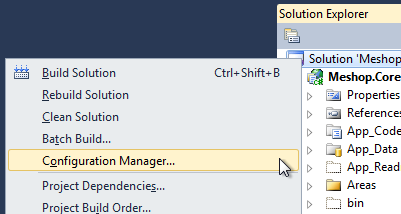
\includegraphics[scale=0.85,angle=0]{figures/build} 
 \caption{Zrušení kompilace Solution}
 \label{fig:build}
 \end{center}
 \end{figure}

\item V otevřeném okně zrušte \textbf{Build} všech projektů.
\item Aplikaci spusťte tlačítkem \textit{Start Debugging} nebo klávesou \textbf{F5}.
\end{enumerate}

Případné problémy při manipulaci s moduly jsou řešeny v kapitole Testování \ref{test:problem}. 

\section{Práce s moduly}
Tvorbu modulů popisuje podrobně sekce Moduly \ref{sec:moduly}. Instalaci modulů pak sekce \ref{sec:instalace}. Problémy s moduly jsou řešeny v kapitole Testování \ref{test:problem}. Vzorová struktura modulu je dostupná v projektu \textsf{Meshop.Reviews}.



%*****************************************************************************
\chapter{Obsah přiloženého DVD}

Na přiloženém DVD je následující adresářová struktura \ref{fig:seznamcd}.

\begin{figure}[h]
\begin{center}
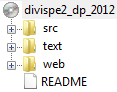
\includegraphics[scale=1]{figures/cd}
\caption{Struktura přiloženého DVD}
\label{fig:seznamcd}
\end{center}
\end{figure}

Soubor \textbf{README} je textový a obsahuje tento text, informace jak aplikaci instalovat, spouštět a jaké požadavky má na hardware.

Adresář \textbf{src} obsahuje kompletní balík projektů (solution). Ten lze otevřít ve Visual Studiu a aplikaci po instalaci všech závislostí spustit přímo v něm.

Adresář \textbf{text} obsahuje soubory s vlastním textem práce v PDF formátu a ve formátu {\LaTeX} s veškerými potřebnými soubory pro kompilaci {\LaTeX} do PDF.

Adresář \textbf{web} obsahuje zkompilovanou aplikaci připravenou pro nasazení na webhosting nebo vlastní IIS server s nainstalovanými závislostmi.

Kompletní obsah DVD je také k dispozici ve webovém repozitáři \url{http://github.com/czechdude/Meshop}, u kterého není vyloučeno, že se časem rozvine v plnohodnotnou aplikaci.



\end{document}
